\documentclass[12pt, a4paper]{report}
\usepackage{graphicx}
\usepackage{geometry}
\geometry{a4paper, margin=1in}
\usepackage{xcolor}
\usepackage{amsmath}
\usepackage{amssymb}
\usepackage{caption}
\usepackage{float}
\usepackage{tikz}
\usepackage{fancyhdr} % For bottom-right page numbers
\usepackage{newtxtext,newtxmath}
\usepackage{inconsolata} % Proper monospace font for code symbols
\usepackage{array}
\usepackage{tabularx}
\newcolumntype{L}[1]{>{\raggedright\arraybackslash}p{#1}}
\newcolumntype{Z}[1]{>{\hsize=#1\hsize\raggedright\arraybackslash}X}

\definecolor{wordblue}{RGB}{46, 116, 181}
\captionsetup[figure]{labelfont=bf}
\captionsetup[table]{labelfont=bf}

% Configure Page Numbers to be Bottom Right
\pagestyle{fancy}
\fancyhf{} 
\renewcommand{\headrulewidth}{0pt}
\fancyfoot[R]{\thepage}

% Force chapter pages to also use bottom right numbers
\fancypagestyle{plain}{
  \fancyhf{}
  \renewcommand{\headrulewidth}{0pt}
  \fancyfoot[R]{\thepage}
}

% --- HYPERREF SETUP ---
% This must be the last package loaded. It makes links clickable and colors them wordblue.
\usepackage{hyperref}
\hypersetup{
    colorlinks=true,
    linkcolor=wordblue,
    citecolor=wordblue,
    urlcolor=wordblue
}
\urlstyle{same}

% Disable italics globally
\renewcommand{\textit}[1]{\textup{#1}}
\renewcommand{\itshape}{\upshape}
\let\it\textup

% Monospace font (inconsolata) is used for code symbols via \texttt

\begin{document}

% ==========================================
% PAGE 1: COVER PAGE (TITLE PAGE)
% ==========================================
\begin{titlepage}
    % This TikZ block draws the thin border on the cover page
    \begin{tikzpicture}[remember picture, overlay]
        \draw[thin] 
            ([xshift=2cm, yshift=-2cm] current page.north west) 
            rectangle 
            ([xshift=-2cm, yshift=2cm] current page.south east);
    \end{tikzpicture}
    
    \begin{center}
        \vspace*{0.5cm}
        
        {\large UNIVERSITY OF SCIENCE AND TECHNOLOGY OF HANOI\par}
        {\large \textbf{DEPARTMENT OF INFORMATION AND COMMUNICATION TECHNOLOGY}\par}
        
        \vspace{2cm}
        
        
\includegraphics[width=0.45\textwidth]{logoUSTH.png}\par
        
        \vspace{2.5cm}
        
        {\Huge \textbf{BACHELOR THESIS}\par}
        
        \vspace{1cm}
        
        {\large By\par}
        \vspace{0.2cm}
        {\Large Nguyễn Phú Vinh\par}
        
        \vspace{1.5cm}
        
        {\large Title:\par}
        \vspace{0.2cm}
        {\LARGE \textbf{Intelligent Job Market Aggregation and\\Analytics Platform}\par}
        
        \vspace{2.5cm}
        
        % Supervisors table aligned nicely
        \begin{tabular}{rl}
            {\large External Supervisor:} & {\large MS Nguyễn Xuân Thịnh} \\
            [0.2cm]
            {\large Internal Supervisor:} & {\large Dr. Giang Anh Tuấn}
        \end{tabular}
        
        \vfill
        
        {\Large \textbf{Hanoi, June 2026}\par}
        
        \vspace*{0.5cm}
    \end{center}
\end{titlepage}

% ==========================================
% PAGE 2: SUPERVISOR'S CERTIFICATE
% ==========================================
\newpage
\pagenumbering{arabic} % Switch to Arabic numerals starting exactly here
\setcounter{page}{1} % Make this explicitly Page 1
\vspace*{3cm}

\begin{center}
    To whom it may concern,
\end{center}

\vspace{1cm}

\noindent I, Nguyễn Xuân Thịnh, certify that the bachelor thesis titled ``Intelligent Job Market Aggregation and Analytics Platform'' submitted by Mr. Nguyễn Phú Vinh is qualified to be presented before the Internship Jury of the academic year 2025-2026.

\vspace{2.5cm}

\begin{flushright}
    Hanoi, June 15, 2026 \\[1.5cm]
    \textbf{Supervisor's signature}
\end{flushright}

\newpage
\addcontentsline{toc}{section}{ACKNOWLEDGEMENTS}
\begin{center}
    {\LARGE \textbf{ACKNOWLEDGEMENTS}\par}
\end{center}
\vspace{1cm}

\noindent I would like to express my deepest gratitude to all those who made it possible for me to complete this bachelor thesis. Foremost, I want to extend my sincere appreciation to my internal and external supervisors for their invaluable guidance, constant encouragement, and insightful feedback throughout the duration of this research. Their expertise in software engineering and machine learning was crucial in steering this project to success.

I am also highly grateful to the Department of Information and Communication Technology at the University of Science and Technology of Hanoi (USTH) for providing a robust academic foundation and supportive environment.

Finally, I would like to thank my family and friends for their unwavering moral support, patience, and encouragement. This work would not have been possible without the collective support of these individuals.

\newpage
\addcontentsline{toc}{section}{LIST OF ABBREVIATIONS}
\begin{center}
    {\LARGE \textbf{LIST OF ABBREVIATIONS}\par}
\end{center}
\vspace{1cm}

\begin{table}[h!]
    \centering
    \normalsize
    \renewcommand{\arraystretch}{1.5}
    \begin{tabularx}{\textwidth}{Z{0.44} | Z{1.56}}
        \textbf{Abbreviation} & \textbf{Expanded Form} \\ \hline
        \textbf{API} & Application Programming Interface \\
        \textbf{BFF} & Backend-For-Frontend \\
        \textbf{ChatML} & Chat Markup Language \\
        \textbf{CRUD} & Create, Read, Update, Delete \\
        \textbf{CUDA} & Compute Unified Device Architecture \\
        \textbf{CV} & Curriculum Vitae \\
        \textbf{DPO} & Direct Preference Optimization \\
        \textbf{ES} & Elasticsearch \\
        \textbf{GPU} & Graphics Processing Unit \\
        \textbf{GridFS} & Grid File System (MongoDB) \\
        \textbf{HNSW} & Hierarchical Navigable Small World \\
        \textbf{HTTP} & Hypertext Transfer Protocol \\
        \textbf{JWT} & JSON Web Token \\
        \textbf{KIE} & Key Information Extraction \\
        \textbf{LLM} & Large Language Model \\
        \textbf{LoRA} & Low-Rank Adaptation \\
        \textbf{ML} & Machine Learning \\
        \textbf{NER} & Named Entity Recognition \\
        \textbf{NLP} & Natural Language Processing \\
        \textbf{OCR} & Optical Character Recognition \\
    \end{tabularx}
\end{table}
\newpage
\begin{table}[h!]
    \centering
    \normalsize
    \renewcommand{\arraystretch}{1.5}
    \begin{tabularx}{\textwidth}{Z{0.44} | Z{1.56}}
        \textbf{Abbreviation} & \textbf{Expanded Form} \\ \hline
        \textbf{PEFT} & Parameter-Efficient Fine-Tuning \\
        \textbf{PII} & Personally Identifiable Information \\
        \textbf{QLoRA} & Quantized Low-Rank Adaptation \\
        \textbf{RAG} & Retrieval-Augmented Generation \\
        \textbf{RLS} & Row Level Security \\
        \textbf{SFT} & Supervised Fine-Tuning \\
        \textbf{SLM} & Small Language Model \\
        \textbf{SPA} & Single Page Application \\
        \textbf{SOTA} & State Of The Art \\
        \textbf{SSR} & Server-Side Rendering \\
        \textbf{TTL} & Time-To-Live \\
        \textbf{VRAM} & Video Random Access Memory \\
    \end{tabularx}
\end{table}

\newpage
\tableofcontents

\newpage
\addcontentsline{toc}{section}{LIST OF TABLES}
\listoftables

\newpage
\addcontentsline{toc}{section}{LIST OF FIGURES}
\listoffigures

\newpage
\addcontentsline{toc}{section}{ABSTRACT}
\begin{center}
    {\LARGE \textbf{ABSTRACT}\par}
\end{center}
\vspace{1cm}

\noindent We present an intelligent, end-to-end Job Market Aggregation and Analytics Platform designed to address the highly fragmented and unstructured nature of the Vietnamese employment market. The platform utilizes automated web scraping pipelines running Playwright to continuously harvest postings from multiple prominent Vietnamese job portals. Structured records are cleaned, normalized using rule-based regular expressions and heuristic natural language processing, and indexed into a high-performance Elasticsearch cluster, enabling sub-100ms full-text search, faceted filtering, and real-time market insights across 6,000+ active job postings. To provide personalized career guidance, we implement a resource-efficient AI chatbot based on a 1.5 billion parameter Small Language Model (SLM), Qwen2.5-1.5B. Using Quantized Low-Rank Adaptation (QLoRA) and Direct Preference Optimization (DPO), we fine-tune three specialized, hot-swappable adapters: a JSON tool caller for intent routing, an empathetic HR coach for CV feedback, and a structured generator for interview matrices. A polyglot persistence architecture utilizing Supabase, Redis, MongoDB, and Qdrant manages user sessions, vector resume embeddings, and conversation logs. Automated evaluation using Gemini-as-a-Judge demonstrates high adapter performance (97.3\% schema extraction accuracy, 98.0\% tool classification accuracy), matching or exceeding models ten times its size. This research proves the viability of deploying fine-tuned, lightweight SLMs for specialized domestic labor market guidance on commodity hardware, offering valuable data-driven tools for Vietnamese students and professionals.

\vspace{1cm}

\noindent Key words: job market analytics, web scraping, Elasticsearch, small language model, QLoRA, DPO, multi-adapter architecture, polyglot persistence, career chatbot, resume parsing, fine-tuning, Vietnam labor market.

\newpage
\begin{center}
    {\Huge \textbf{Chapter 1: Introduction and Contributions}\par}
\end{center}
\vspace{1cm}
\addcontentsline{toc}{chapter}{Chapter 1: Introduction and Contributions}

\addcontentsline{toc}{section}{1.1 Global Context \& Motivation}
\noindent{\LARGE \textbf{1.1 Global Context \& Motivation}\par}
\vspace{0.4cm}

\setlength{\parindent}{0.7cm}
\setlength{\parskip}{0.1cm}

In recent years, the rapid growth of the digital economy has transformed the global and domestic labor markets. Vietnam, as a fast-emerging market, has experienced a significant surge in demand for high-skilled labor, particularly in information technology, digital marketing, and financial services [\hyperlink{cite11}{11}]. However, the domestic job market remains highly fragmented. Job postings are scattered across dozens of disconnected online employment portals (such as TopCV, VietnamWorks, and JobOKO), each using proprietary classifications, diverse salary formatting, and varying descriptions. This fragmentation creates search friction for job seekers who must manually browse multiple websites, compile matching data, and evaluate their own qualifications against inconsistent requirement definitions.

For students and young professionals entering this dynamic landscape, the challenge is twofold. First, they lack centralized, real-time analytics to understand broader market demands-such as which skills are most sought after, how salaries are distributed across regions, or which sectors are expanding. Second, they lack access to personalized, expert career guidance. Traditional career consulting is either prohibitively expensive or generic, while existing automated resume screening tools (often based on basic keyword matching) fail to provide actionable, constructive feedback for candidates to improve their resumes and bridge skill gaps.

This research is motivated by the potential of combining web automation, information retrieval, and modern artificial intelligence to build a unified, intelligent analytics platform. By combining automated data aggregation with local large language model (LLM) inference, we can create a system that not only indexes and visualizes market trends in real time but also serves as an interactive, resume-aware career assistant. Such a platform democratizes career guidance, helping candidates optimize their market readiness.

\vspace{0.8cm}
\addcontentsline{toc}{section}{1.2 Problem Statement}
\noindent{\LARGE \textbf{1.2 Problem Statement}\par}
\vspace{0.4cm}

Despite these advancements, existing Vietnamese career portals and recruitment tools exhibit three main technical limitations:

\begin{enumerate}
    \item Fragmented and Unstructured Data Sources: Web-scraped data from Vietnamese job sites is extremely noisy, with unstructured salary ranges, non-standardized skill names, and duplicate postings [\hyperlink{cite14}{14}]. Traditional classification algorithms and regex-based heuristics often struggle to structure Vietnamese job postings accurately due to syntax complexity, spelling variations, and mixed English-Vietnamese terminology.
    \item High Resource Demands for Intelligent Chatbots: Deploying interactive, conversational career agents usually requires querying expensive, external cloud APIs or hosting massive models. This introduces high API dependencies and operating costs that can restrict accessibility for local educational or public organizations, and poses privacy risks when processing personal Curriculum Vitae (CV) documents.
    \item Task Drift in Single-Prompt SLMs: A single parameter-efficient small language model (SLM) under 2 billion parameters struggles to generalize across multiple heterogeneous tasks (e.g., intent classification, prose coaching, structured data formatting) within a single prompt context, resulting in format drift and loss of coherence.
\end{enumerate}

\vspace{0.8cm}
\addcontentsline{toc}{section}{1.3 Research Questions}
\noindent{\LARGE \textbf{1.3 Research Questions}\par}
\vspace{0.4cm}

To address these limitations, this thesis investigates the following key research questions:

\begin{enumerate}
    \item RQ1: How can we design an automated data collection and processing pipeline that crawls, cleans, and normalizes unstructured Vietnamese job postings into a high-quality standardized schema using rule-based regular expressions and heuristic natural language processing?
    \item RQ2: How can we design a polyglot persistence and retrieval architecture that enables both high-performance, low-latency full-text job search and aspect-specific vector-based resume matching?
    \item RQ3: How can we build a resource-efficient, local conversational agent using a multi-adapter SLM architecture that matches the task-specific schema extraction and intent routing accuracy of larger commercial LLMs while running on commodity hardware?
\end{enumerate}

\vspace{0.8cm}
\addcontentsline{toc}{section}{1.4 Scientific and Technical Contributions}
\noindent{\LARGE \textbf{1.4 Scientific and Technical Contributions}\par}
\vspace{0.4cm}

This thesis makes three primary scientific and technical contributions to the field of intelligent recruitment aggregation and local AI coaching:

\begin{enumerate}
    \item We design and implement an end-to-end data acquisition and normalization pipeline tailored for the Vietnamese job market, utilizing Playwright for robust dynamic crawling and a hybrid extraction framework that achieves an 85.3\% validation rate.
    \item We construct a production-ready polyglot persistence layer (combining MongoDB, Redis, Elasticsearch, and Qdrant) that manages caching, session history, full-text faceted search, and resume vector embeddings, maintaining sub-50ms median query latency under loads of up to 50 concurrent requests.
    \item We propose a resource-efficient local conversational agent based on a multi-adapter SLM architecture. By fine-tuning task-specific QLoRA adapters on Qwen2.5-1.5B and applying DPO alignment, we show that a lightweight model can run locally on consumer hardware while matching the task-specific performance of commercial models ten times its size.
\end{enumerate}

\newpage
\begin{center}
    {\Huge \textbf{Chapter 2: Objective and Literature Review}\par}
\end{center}
\vspace{1cm}
\addcontentsline{toc}{chapter}{Chapter 2: Objective and Literature Review}

\addcontentsline{toc}{section}{2.1 Research Objectives}
\noindent{\LARGE \textbf{2.1 Research Objectives}\par}
\vspace{0.4cm}

\setlength{\parindent}{0.7cm}
\setlength{\parskip}{0.1cm}

The primary objective of this research is to design, implement, and evaluate an intelligent, end-to-end Job Market Aggregation and Analytics Platform that automates the collection and standardization of Vietnamese job listings, combines high-performance full-text search with real-time market analytics, and deploys a local, privacy-preserving AI career assistant powered by a multi-adapter Small Language Model (SLM). To achieve this, we propose a modular architecture comprising automated multi-source web scraping [\hyperlink{cite10}{10}], heuristic-driven data normalization, sub-100ms Elasticsearch retrieval [\hyperlink{cite2}{2}], and three task-specific QLoRA adapters [\hyperlink{cite4}{4}, \hyperlink{cite5}{5}] on a shared Qwen2.5-1.5B base model [\hyperlink{cite7}{7}], orchestrated within a containerized polyglot persistence infrastructure [\hyperlink{cite12}{12}, \hyperlink{cite13}{13}].

\vspace{0.8cm}
\addcontentsline{toc}{section}{2.2 Literature Review}
\noindent{\LARGE \textbf{2.2 Literature Review}\par}
\vspace{0.4cm}

\addcontentsline{toc}{subsection}{2.2.1 Web Scraping and Data Normalization in HR Tech}
\noindent{\Large \textbf{2.2.1 Web Scraping and Data Normalization in HR Tech}\par}
\vspace{0.4cm}

Web scraping is a standard method for aggregating employment data in research and industry. Traditional crawlers rely on libraries like BeautifulSoup or Scrapy. However, modern job portals increasingly utilize Single Page Application (SPA) architectures and anti-bot defenses (such as dynamic DOM rendering, rate limits, and browser fingerprinting). This has shifted the state-of-the-art toward automated browser frameworks like Playwright [\hyperlink{cite10}{10}] and Puppeteer, which run headless Chromium instances to simulate human interactions.

Once scraped, the raw text remains unstructured and noisy. Standard normalization techniques rely on rule-based regular expressions and heuristic natural language processing parsing frameworks to clean salary formats, categorize locations, and extract job schemas. These rule-based parsing approaches offer highly predictable, deterministic transformations, making them ideal for high-throughput, low-latency ingestion pipelines. For Vietnamese text processing, an Electra-based pre-trained model (specifically NlpHUST's ner-vietnamese-electra-base [\hyperlink{cite8}{8}]) enables domain-specific NER on Vietnamese documents, extracting named entities (persons, organizations, locations) that complement rule-based approaches. Server-side orchestration of these cleaning and processing pipelines is increasingly handled by high-performance Python API frameworks such as FastAPI [\hyperlink{cite15}{15}].

\vspace{0.6cm}
\addcontentsline{toc}{subsection}{2.2.2 Full-Text Search and Vector Retrieval}
\noindent{\Large \textbf{2.2.2 Full-Text Search and Vector Retrieval}\par}
\vspace{0.4cm}

To navigate large-scale job databases, efficient search engines are required. Lucene-based search clusters, notably Elasticsearch, serve as the standard for full-text search [\hyperlink{cite2}{2}]. They support multi-field querying, BM25 text relevance scoring, and faceted filter aggregations, enabling sub-second search times across millions of records.

However, keyword search is limited by semantic vocabulary mismatch (e.g., searching ``Frontend'' might miss ``React developer''). This has led to the adoption of vector-based similarity search using dense embeddings (e.g., BGE-M3, Sentence-BERT) indexed in specialized vector databases like Qdrant, following the Retrieval-Augmented Generation (RAG) paradigm [\hyperlink{cite6}{6}]. In this platform, only resume documents are encoded as high-dimensional vectors in Qdrant to enable aspect-scoped semantic matching and skill-gap calculations, whereas job descriptions are indexed directly in Elasticsearch (full-text search) and matched via keyword/token overlap rather than job vector indexing.

\vspace{0.6cm}
\addcontentsline{toc}{subsection}{2.2.3 Parameter-Efficient Fine-Tuning and SLMs}
\noindent{\Large \textbf{2.2.3 Parameter-Efficient Fine-Tuning and SLMs}\par}
\vspace{0.4cm}

Although giant LLMs (e.g., GPT-4, Llama-3-70B) demonstrate impressive capabilities, deploying them in production presents severe challenges. They require costly, high-end cloud GPU infrastructure, introduce data privacy concerns, and exhibit high latency. Consequently, there is growing academic interest in Small Language Models (SLMs) with under 3 billion parameters, such as Qwen2.5-1.5B [\hyperlink{cite7}{7}] or Gemma-2B, which can run locally on consumer-grade hardware.

To match the task performance of larger models, SLMs are adapted using Parameter-Efficient Fine-Tuning (PEFT) techniques, particularly Low-Rank Adaptation (LoRA) and its quantized variant, QLoRA [\hyperlink{cite4}{4}]. QLoRA quantizes the base model's weights into 4-bit representation to minimize memory footprint, injecting lightweight trainable low-rank adapters. Direct Preference Optimization (DPO) further aligns model outputs with specific human guidelines (such as consulting tone and formatting constraints) by optimizing directly on pairwise preferences, bypassing the complexity of reinforcement learning with human feedback (RLHF) [\hyperlink{cite9}{9}].

A key architectural question is whether to use a single general-purpose model or to decompose tasks across multiple specialized adapters. Recent work on multi-adapter composition has demonstrated that mounting multiple lightweight LoRA adapters on a shared base model can achieve task-specific accuracy comparable to much larger monolithic models, while dramatically reducing inference-time resource requirements [\hyperlink{cite16}{16}]. This adapter-switching paradigm avoids the catastrophic forgetting that typically occurs when a single small model is fine-tuned on heterogeneous tasks. Furthermore, synthetic data generation has emerged as a practical methodology for training domain-specific NLP models, particularly in contexts where real-world data is scarce, sensitive, or lacks ground-truth annotations [\hyperlink{cite17}{17}]. Teacher-student distillation frameworks, where a large LLM generates training data that is subsequently used to fine-tune a smaller student model, have proven effective across classification, summarization, and structured generation tasks [\hyperlink{cite18}{18}].

\newpage
\begin{center}
    {\Huge \textbf{Chapter 3: Materials and Methods}\par}
\end{center}
\vspace{1cm}
\addcontentsline{toc}{chapter}{Chapter 3: Materials and Methods}

\setlength{\parindent}{0.7cm}
\setlength{\parskip}{0.1cm}

This chapter presents the complete system architecture across five interconnected subsystems. Section 3.1 introduces the high-level AI orchestration and container topology that organizes the platform into three computational domains. Section 3.2 details the polyglot persistence layer and its four-database topology for managing session state, conversation history, vector embeddings, and user profiles. Section 3.3 describes the frontend presentation layer and its server-client rendering boundary. Section 3.4 documents the AI chatbot orchestrator and its multi-adapter Small Language Model inference engine. Finally, Section 3.5 presents the offline ML training pipeline that produces and aligns the three task-specific QLoRA adapters.

\vspace{0.8cm}
\addcontentsline{toc}{section}{3.1 AI Orchestration \& ML Pipeline Architecture}
\noindent{\LARGE \textbf{3.1 AI Orchestration \& ML Pipeline Architecture}\par}
\vspace{0.4cm}

\addcontentsline{toc}{subsection}{3.1.1 Overview}
\noindent{\Large \textbf{3.1.1 Overview}\par}
\vspace{0.4cm}

\setlength{\parindent}{0.7cm}
\setlength{\parskip}{0.1cm}

The CareerIntel platform is built around a central architectural premise: a small language model (SLM) with only 1.5 billion parameters can match or exceed the task-specific performance of models ten times its size - provided that its responsibilities are decomposed into discrete, fine-tuned sub-tasks rather than handled by a single general-purpose prompt. This premise drives every layer of the system, from the three-adapter inference engine that serves users in real time, to the six-phase training pipeline that produces those adapters, to the polyglot persistence layer that maintains conversational state across sessions.

This chapter presents the high-level architecture of the AI components: the computational domains that organize the system, the container topology that isolates them, the key design tradeoffs that shape their interaction, and the end-to-end data flows that connect a user's request to an AI-generated response. Subsequent sections elaborate each domain in depth \textemdash{} \S3.2 details the persistence layer, \S3.4 describes the multi-adapter inference engine, and \S3.5 documents the training pipeline.

\vspace{0.6cm}
\addcontentsline{toc}{subsection}{3.1.2 Three-Domain Architecture}
\noindent{\Large \textbf{3.1.2 Three-Domain Architecture}\par}
\vspace{0.4cm}

The AI subsystem is organized into three computational domains, each with distinct latency requirements, resource profiles, and failure characteristics. This separation ensures that heavy tensor computations do not block real-time user interactions, and that persistent state remains durable independently of the compute layer's lifecycle.

\vspace{0.4cm}
\noindent{\large \textbf{3.1.2.1 Synchronous Inference Domain}\par}
\vspace{0.3cm}

The synchronous inference domain handles the real-time chat loop: receiving a user message, classifying intent, routing to the appropriate adapter, generating a response, and returning it - all within the latency budget of a single HTTP request-response cycle. Two components collaborate in this domain:

\begin{itemize}
    \item FastAPI Orchestrator - the central coordinator that exposes chat and upload endpoints, manages session state, and implements the tool dispatch decision tree. It determines \textit{which} adapter should handle each request and \textit{how} the response should be framed, but delegates the actual text generation to the inference engine.
    \item Ollama Inference Engine - hosts three QLoRA-finetuned adapters on the same Qwen2.5:1.5B base model, each specialized for a different output modality: structured JSON for intent classification (Adapter A), empathetic Vietnamese prose for career coaching (Adapter B), and formatted markdown tables for interview preparation (Adapter C). All three adapters share the base model's weights in memory, with only lightweight LoRA delta matrices differentiating them.
\end{itemize}

The critical design decision in this domain is that Ollama runs natively on the host machine rather than inside a container. This hybrid approach allows the inference engine to access host GPU hardware directly, avoiding the configuration complexity of Docker GPU passthrough while keeping all application logic fully containerized.

\vspace{0.4cm}
\noindent{\large \textbf{3.1.2.2 Asynchronous Extraction Domain}\par}
\vspace{0.3cm}

CV processing - parsing PDFs, running Named Entity Recognition, computing vector embeddings - routinely takes 30 to 180 seconds, far exceeding acceptable synchronous response times. The asynchronous domain isolates these heavy workloads behind a task queue:

\begin{itemize}
    \item Celery Worker - a background processor that consumes extraction tasks from a Redis-backed message queue. It executes the same three-stage extraction cascade used in the training pipeline (semantic chunking $\rightarrow$ regex extraction $\rightarrow$ Electra NER), followed by quality scoring and BGE-M3 embedding generation. Machine learning models are pre-warmed at worker startup, eliminating the approximately 50-second cold-start penalty on the first upload.
    \item Redis Broker - mediates between the FastAPI orchestrator (which dispatches tasks) and the Celery worker (which executes them), decoupling request acceptance from processing completion.
\end{itemize}

The frontend observes extraction progress through a long-polling pattern: the backend returns a job identifier immediately upon upload, and the client polls a status endpoint every two seconds until the worker reports completion.

\vspace{0.4cm}
\noindent{\large \textbf{3.1.2.3 Persistent Intelligence Domain}\par}
\vspace{0.3cm}

The persistence layer spans four specialized databases, each chosen for a distinct access pattern that no single database could serve optimally:

\begin{itemize}
    \item Redis - in-memory cache for active session data (resume bindings, recent conversation turns) with 24-hour TTL-based eviction. Serves as the first-read tier in a three-level fallback chain.
    \item MongoDB - durable store for conversation history, session metadata, and raw uploaded files (via GridFS). Provides the source-of-truth for session restoration after Redis eviction.
    \item Qdrant - vector database storing 1024-dimensional BGE-M3 embeddings across four named vectors per resume (full\_profile, skills, experience, education), enabling aspect-specific semantic search and skill-gap analysis.
    \item Supabase (PostgreSQL) - persistent, user-scoped resume storage that survives across chatbot sessions. A three-tier fallback chain (Redis $\rightarrow$ MongoDB $\rightarrow$ Supabase) ensures returning users can access their resume data without re-uploading.
\end{itemize}

This polyglot strategy reflects a deliberate architectural trade: operational complexity in managing four databases is accepted in exchange for each database serving its optimal access pattern - sub-millisecond reads from Redis, flexible document queries from MongoDB, high-dimensional similarity search from Qdrant, and relational integrity with Row Level Security from PostgreSQL.

\begin{figure}[H]
    \centering
    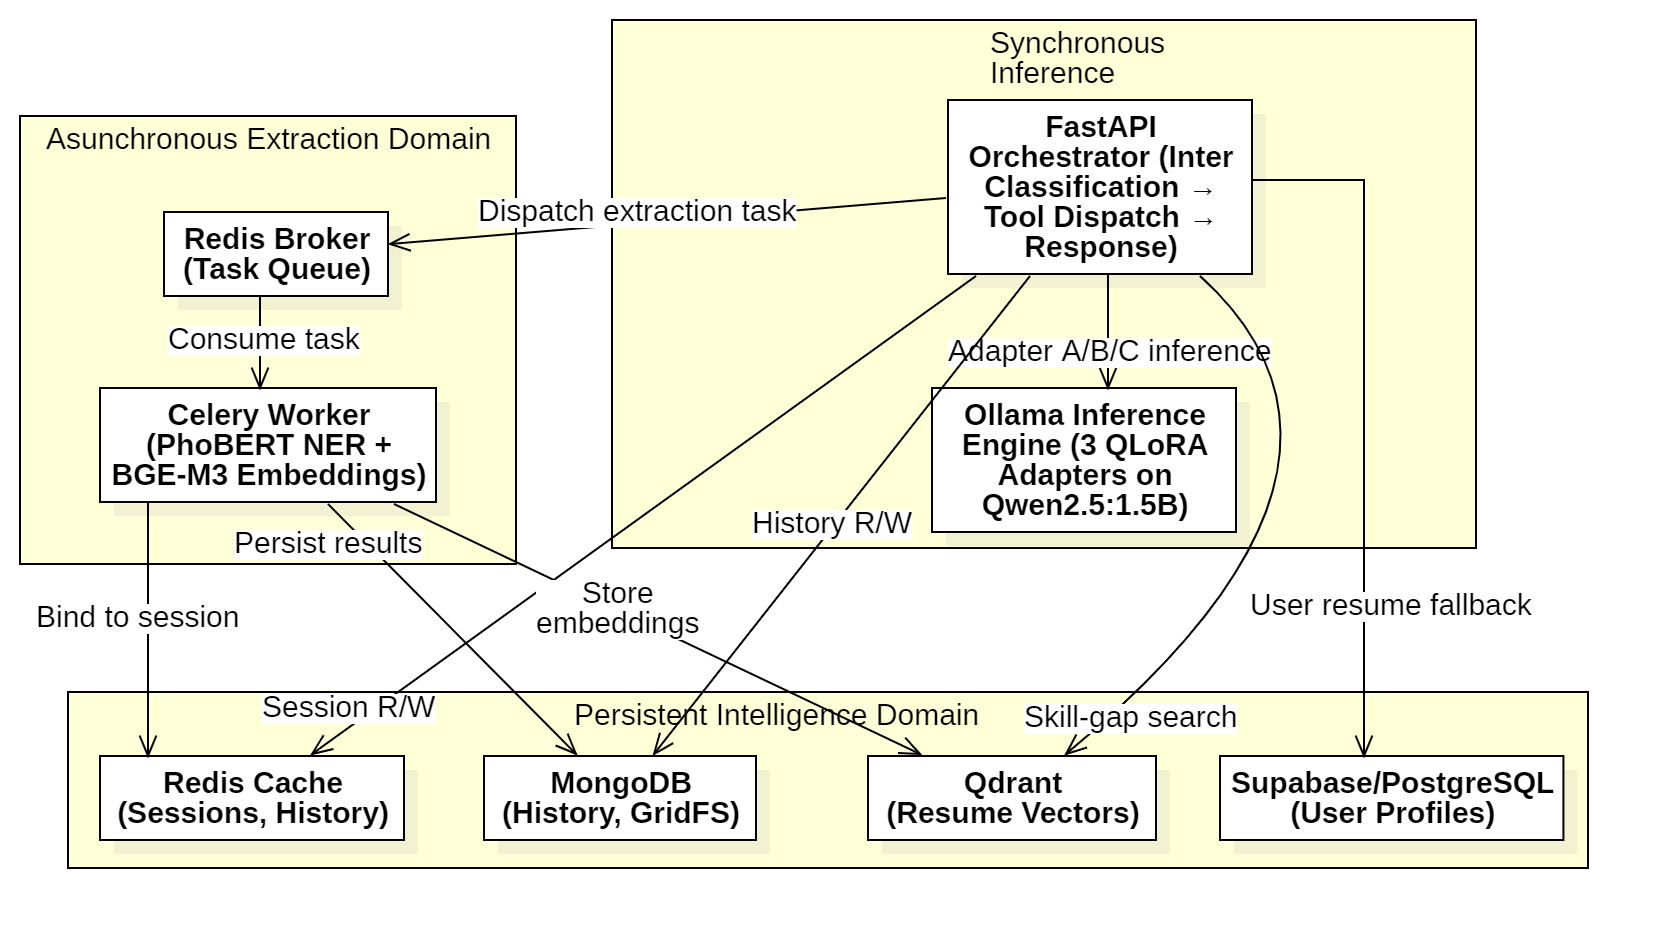
\includegraphics[width=0.85\textwidth]{thesis_1_images/chapter_1_thesis_1_diagram_1.png}
    \caption[Three-domain AI subsystem architecture]{\textbf{Three-domain AI subsystem architecture}: \textmd{The three computational domains (synchronous inference, asynchronous extraction, and persistent intelligence) work together to manage requests.}}
\end{figure}

\vspace{0.6cm}
\addcontentsline{toc}{subsection}{3.1.3 Container Topology}
\noindent{\Large \textbf{3.1.3 Container Topology}\par}
\vspace{0.4cm}

The system is deployed as a Docker Compose cluster comprising seven containers organized into three functional tiers, plus the Ollama inference engine running natively on the host. The containerization boundary is drawn precisely at the point where GPU access is required: all application logic, databases, and background workers run inside containers, while the inference engine that requires direct hardware access runs outside.

\begin{figure}[H]
    \centering
    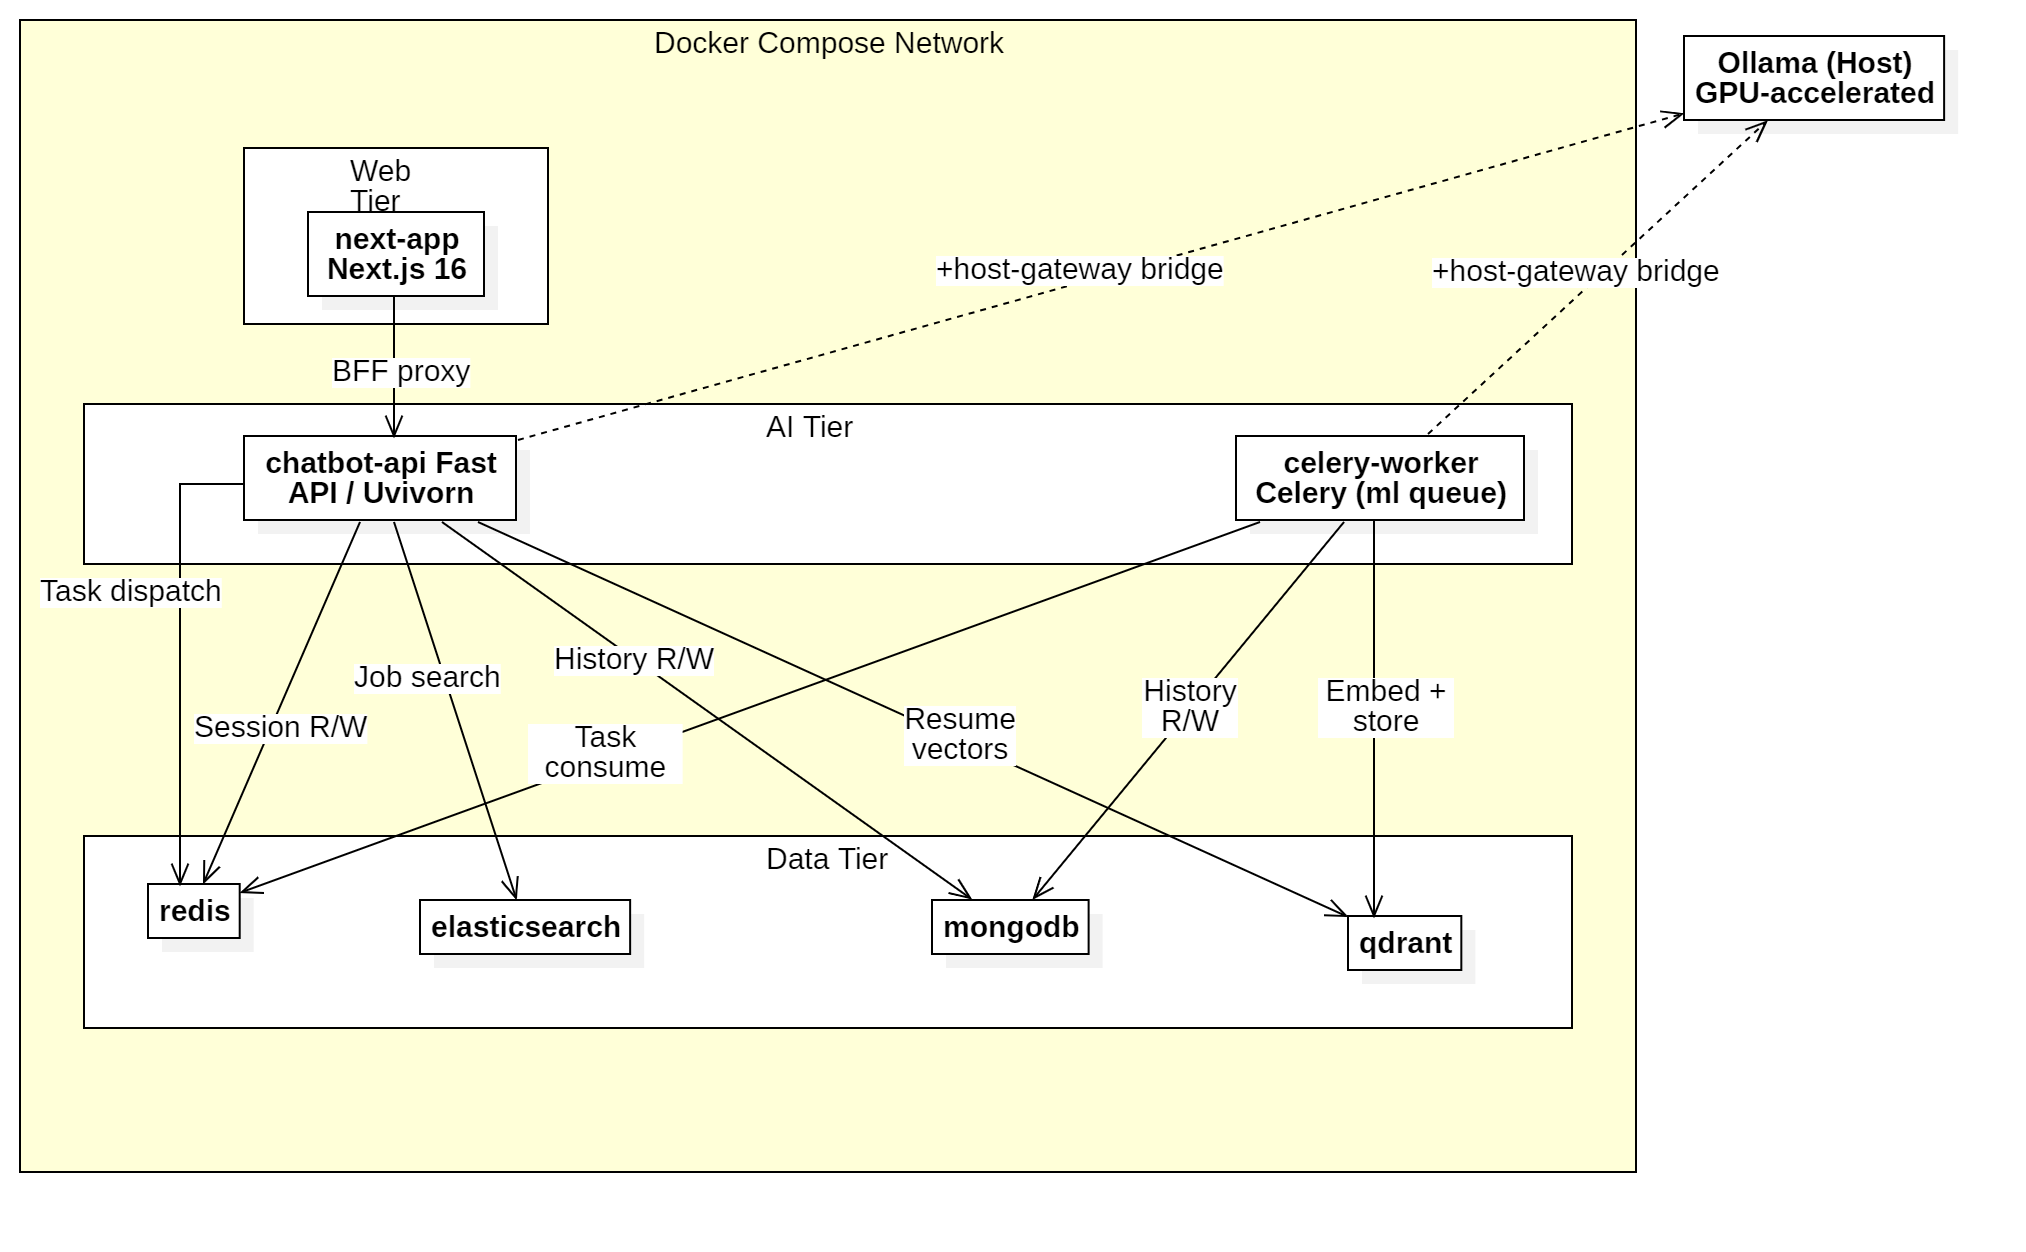
\includegraphics[width=0.85\textwidth]{thesis_1_images/chapter_1_thesis_1_diagram_2.png}
    \caption[Container topology of the Docker Compose services]{\textbf{Container topology of the Docker Compose services}: \textmd{Seven microservices are isolated inside a custom Docker network with automated health checks.}}
\end{figure}

The Next.js frontend communicates with the FastAPI orchestrator exclusively through a Backend-For-Frontend (BFF) proxy layer, which normalizes upstream errors and ensures the backend is never directly exposed to the public network. The dashed lines to the Ollama node represent the host-gateway DNS bridge described in §3.1.4.1.

Docker Compose orchestrates the startup sequence through a health-gated dependency graph: data-tier services (Redis, MongoDB, Elasticsearch) must pass their health probes before AI-tier services are permitted to start, preventing connection failures during initialization. Qdrant uses a weaker \texttt{service\_started} condition because the Celery worker lazily initializes its Qdrant client only upon the first CV upload, tolerating a brief startup window.

\vspace{0.6cm}
\addcontentsline{toc}{subsection}{3.1.4 Design Tradeoffs}
\noindent{\Large \textbf{3.1.4 Design Tradeoffs}\par}
\vspace{0.4cm}

\vspace{0.4cm}
\noindent{\large \textbf{3.1.4.1 CPU Containers with Host GPU Bridge}\par}
\vspace{0.3cm}

Running fine-tuned language models requires GPU hardware, yet configuring Docker GPU passthrough (via the Nvidia Container Toolkit) introduces significant operational complexity - driver version dependencies, runtime configuration, and potential conflicts with host processes. The architecture resolves this tension through a hybrid deployment: the Ollama inference engine runs natively on the host machine with direct GPU access, while the application logic remains fully containerized with CPU-only images.

Communication between containerized services and the host inference engine is established via Docker's DNS resolution mechanism (\texttt{host.docker.internal}), which resolves to the host machine's gateway address. This allows both the FastAPI orchestrator and the Celery worker to invoke Ollama's API without leaving the Docker network's logical boundary.

The container images are built from \texttt{python:3.11-slim} and explicitly target CPU-only PyTorch wheels, omitting the approximately 2 GB of CUDA runtime libraries that would otherwise bloat each image. System-level OCR dependencies (Tesseract with Vietnamese language support) are installed at build time, ensuring that scanned-document processing is available without additional host configuration.

This tradeoff yields a clean separation of concerns: containers encapsulate application dependencies and can be reproduced identically across development machines, while the host retains exclusive control over GPU resource allocation and model loading.

\vspace{0.4cm}
\noindent{\large \textbf{3.1.4.2 Zero-Copy File Exchange}\par}
\vspace{0.3cm}

A fundamental bottleneck in distributed ML pipelines involving large file payloads is the serialization overhead of pushing binary data through a message broker. A 10 MB PDF encoded as Base64 expands to approximately 13.3 MB and must be serialized into a Redis message, transmitted, deserialized, and decoded - consuming broker memory and adding latency proportional to file size.

CareerIntel eliminates this overhead through a zero-copy exchange pattern using a shared Docker volume (\texttt{shared\_tmp}):

\begin{figure}[H]
    \centering
    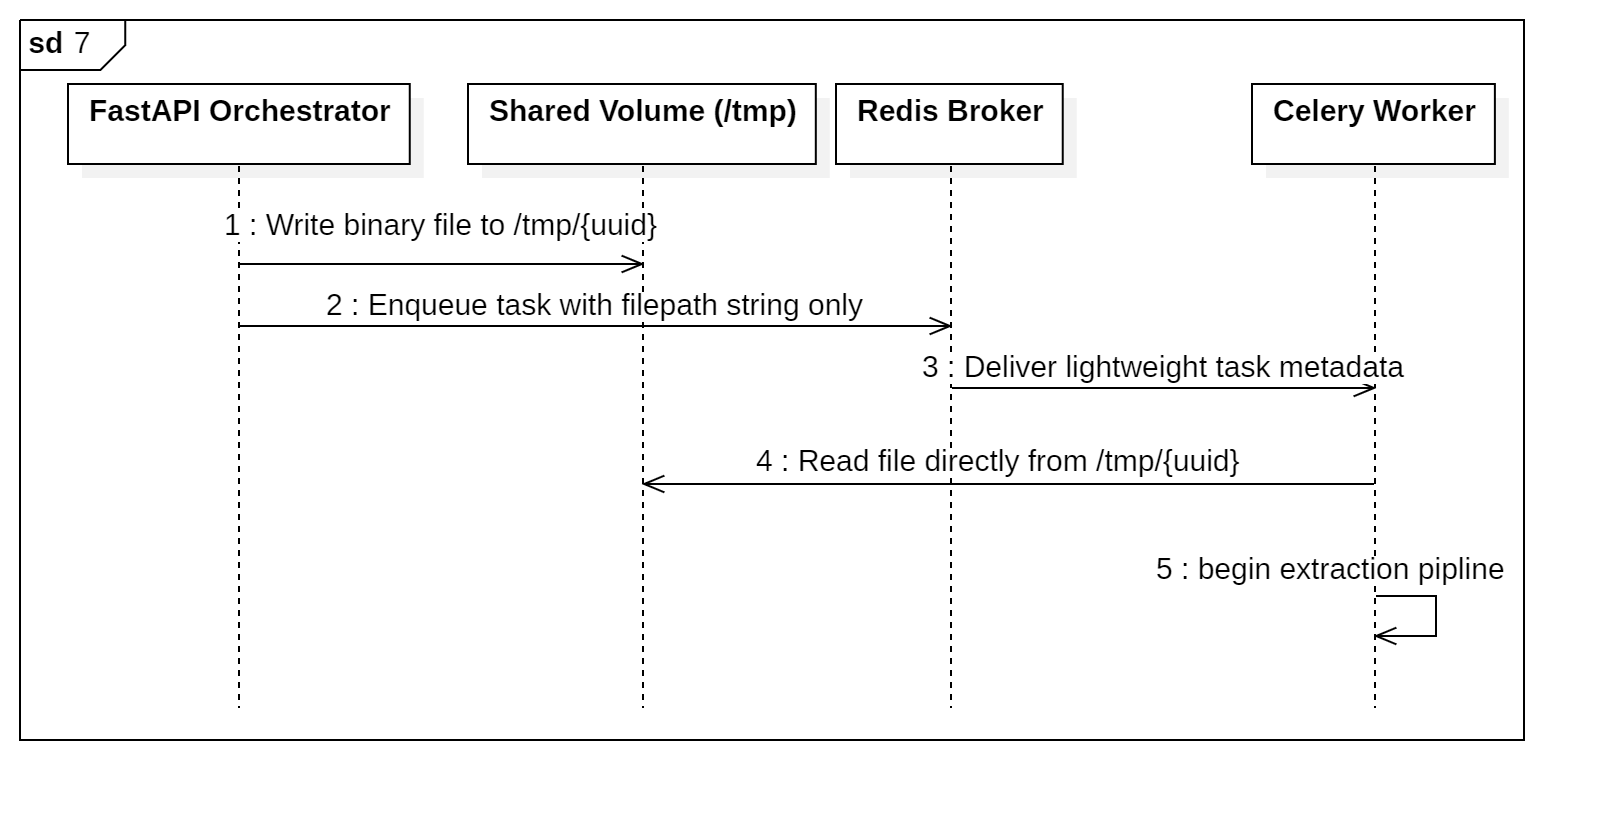
\includegraphics[width=0.85\textwidth]{thesis_1_images/chapter_1_thesis_1_diagram_3.png}
    \caption[Zero-copy file exchange sequence diagram]{\textbf{Zero-copy file exchange sequence diagram}: \textmd{The orchestrator writes binary files to a shared volume to eliminate serialization overhead.}}
\end{figure}

The orchestrator writes the uploaded file to the shared volume and enqueues only the filepath string (tens of bytes) through Redis, rather than the file content (megabytes). The worker reads the file directly from the same volume mount, achieving zero serialization overhead regardless of file size. This pattern reduces broker memory pressure and eliminates the Base64 encoding/decoding latency entirely.

\vspace{0.6cm}
\addcontentsline{toc}{subsection}{3.1.5 Request Lifecycle Flows}
\noindent{\Large \textbf{3.1.5 Request Lifecycle Flows}\par}
\vspace{0.4cm}

\vspace{0.4cm}
\noindent{\large \textbf{3.1.5.1 Chat Request Pipeline}\par}
\vspace{0.3cm}

Every chat interaction traverses a nine-step pipeline that transforms a natural-language user message into an adapter-generated response. The pipeline demonstrates how the three computational domains collaborate at runtime:

\begin{figure}[H]
    \centering
    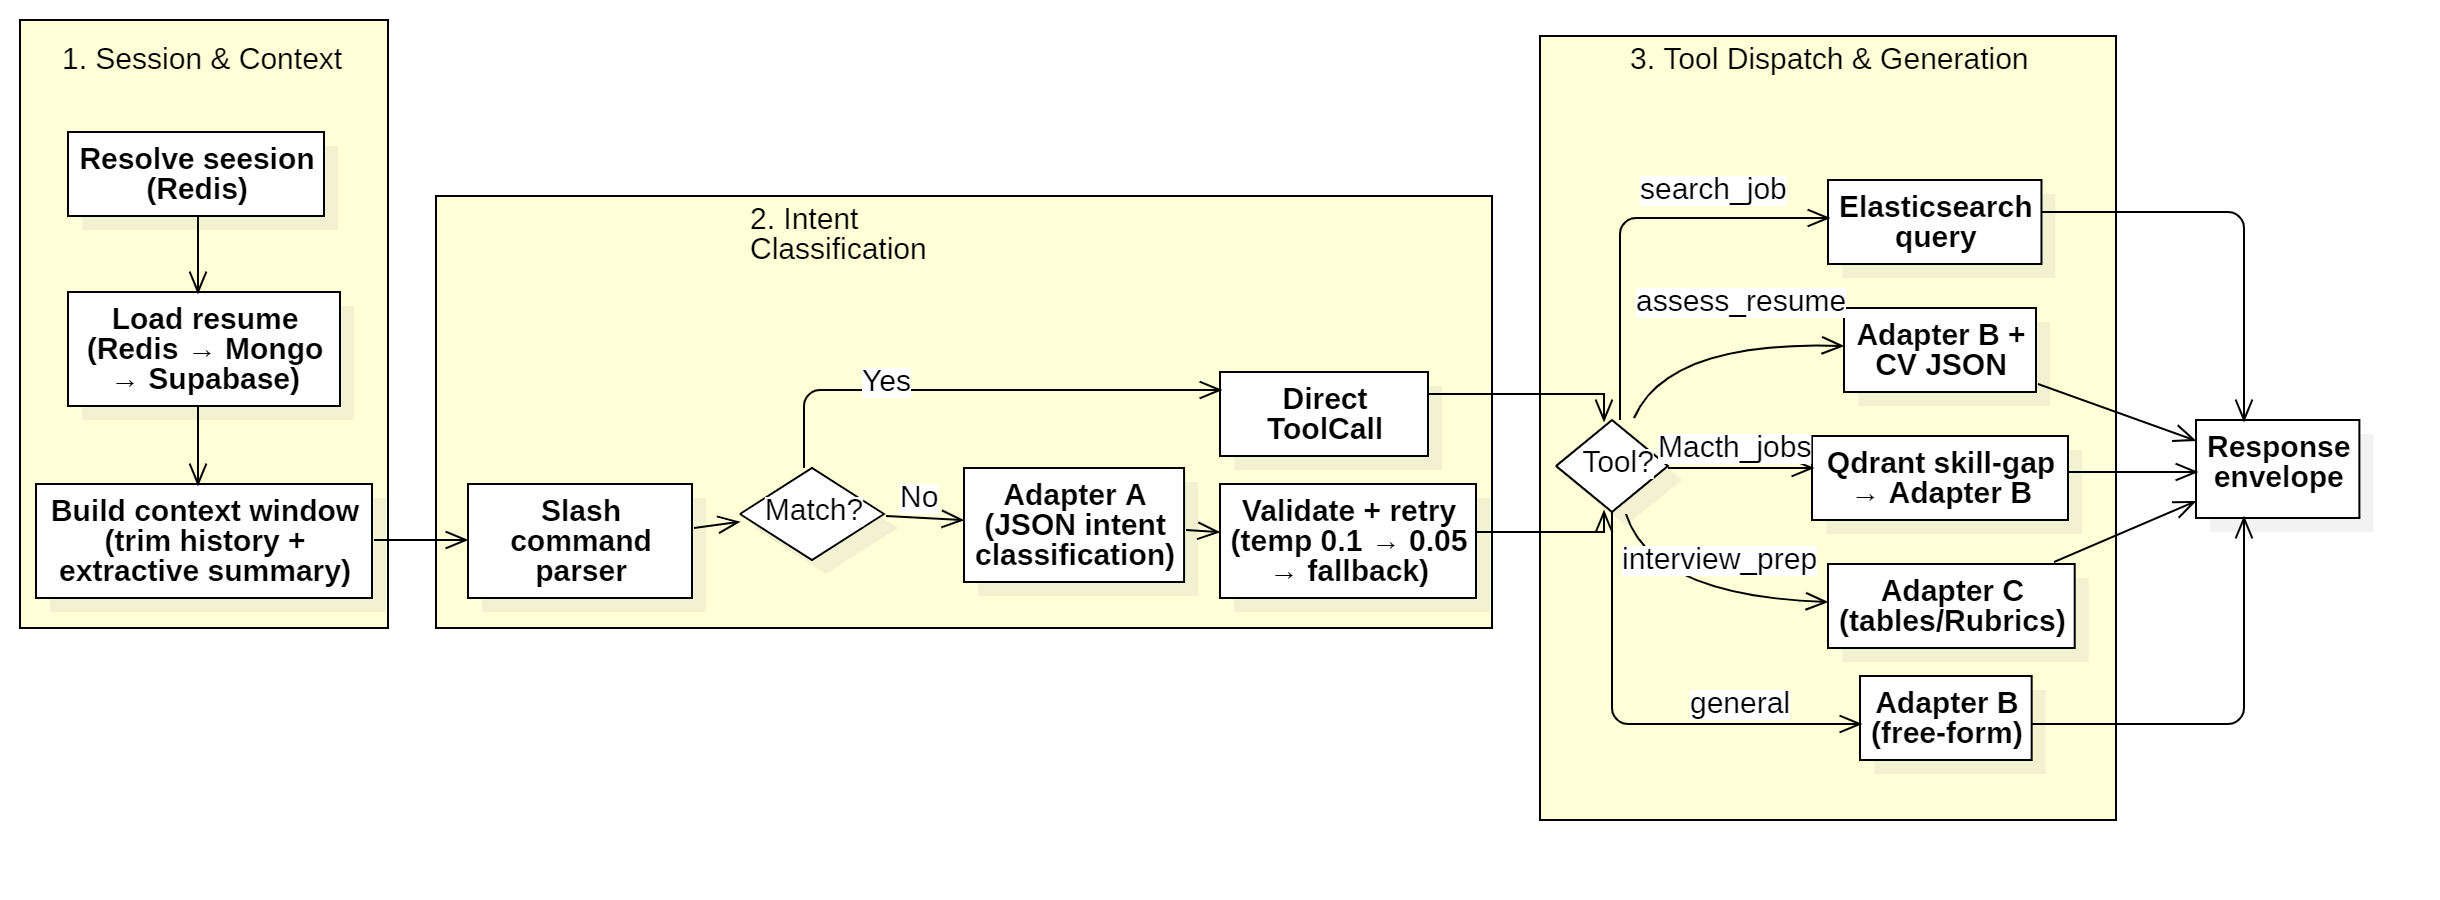
\includegraphics[width=0.85\textwidth]{thesis_1_images/chapter_1_thesis_1_diagram_4.png}
    \caption[Chat request pipeline flowchart]{\textbf{Chat request pipeline flowchart}: \textmd{Natural-language requests are routed through Adapter A for intent routing, followed by adapter dispatch or database search.}}
\end{figure}

The pipeline begins in the Persistent Intelligence Domain (session resolution, history retrieval, context window management), transitions through Adapter A's intent classification in the Synchronous Inference Domain, and branches into five execution paths - one of which (job search) queries Elasticsearch directly without invoking a language model, while the remaining four route through Adapters B or C for text generation.

A critical architectural feature is the retry-with-temperature-drop strategy for intent classification: if Adapter A's initial response fails JSON validation, the system retries at near-greedy temperature (0.05) before gracefully degrading to a general conversational response. This three-tier resilience ensures users always receive a meaningful reply, even when intent classification is uncertain.

\vspace{0.4cm}
\noindent{\large \textbf{3.1.5.2 CV Upload Pipeline}\par}
\vspace{0.3cm}

The CV upload flow demonstrates the data transformation chain that converts an unstructured document into a structured, searchable, AI-ready representation:

\begin{figure}[H]
    \centering
    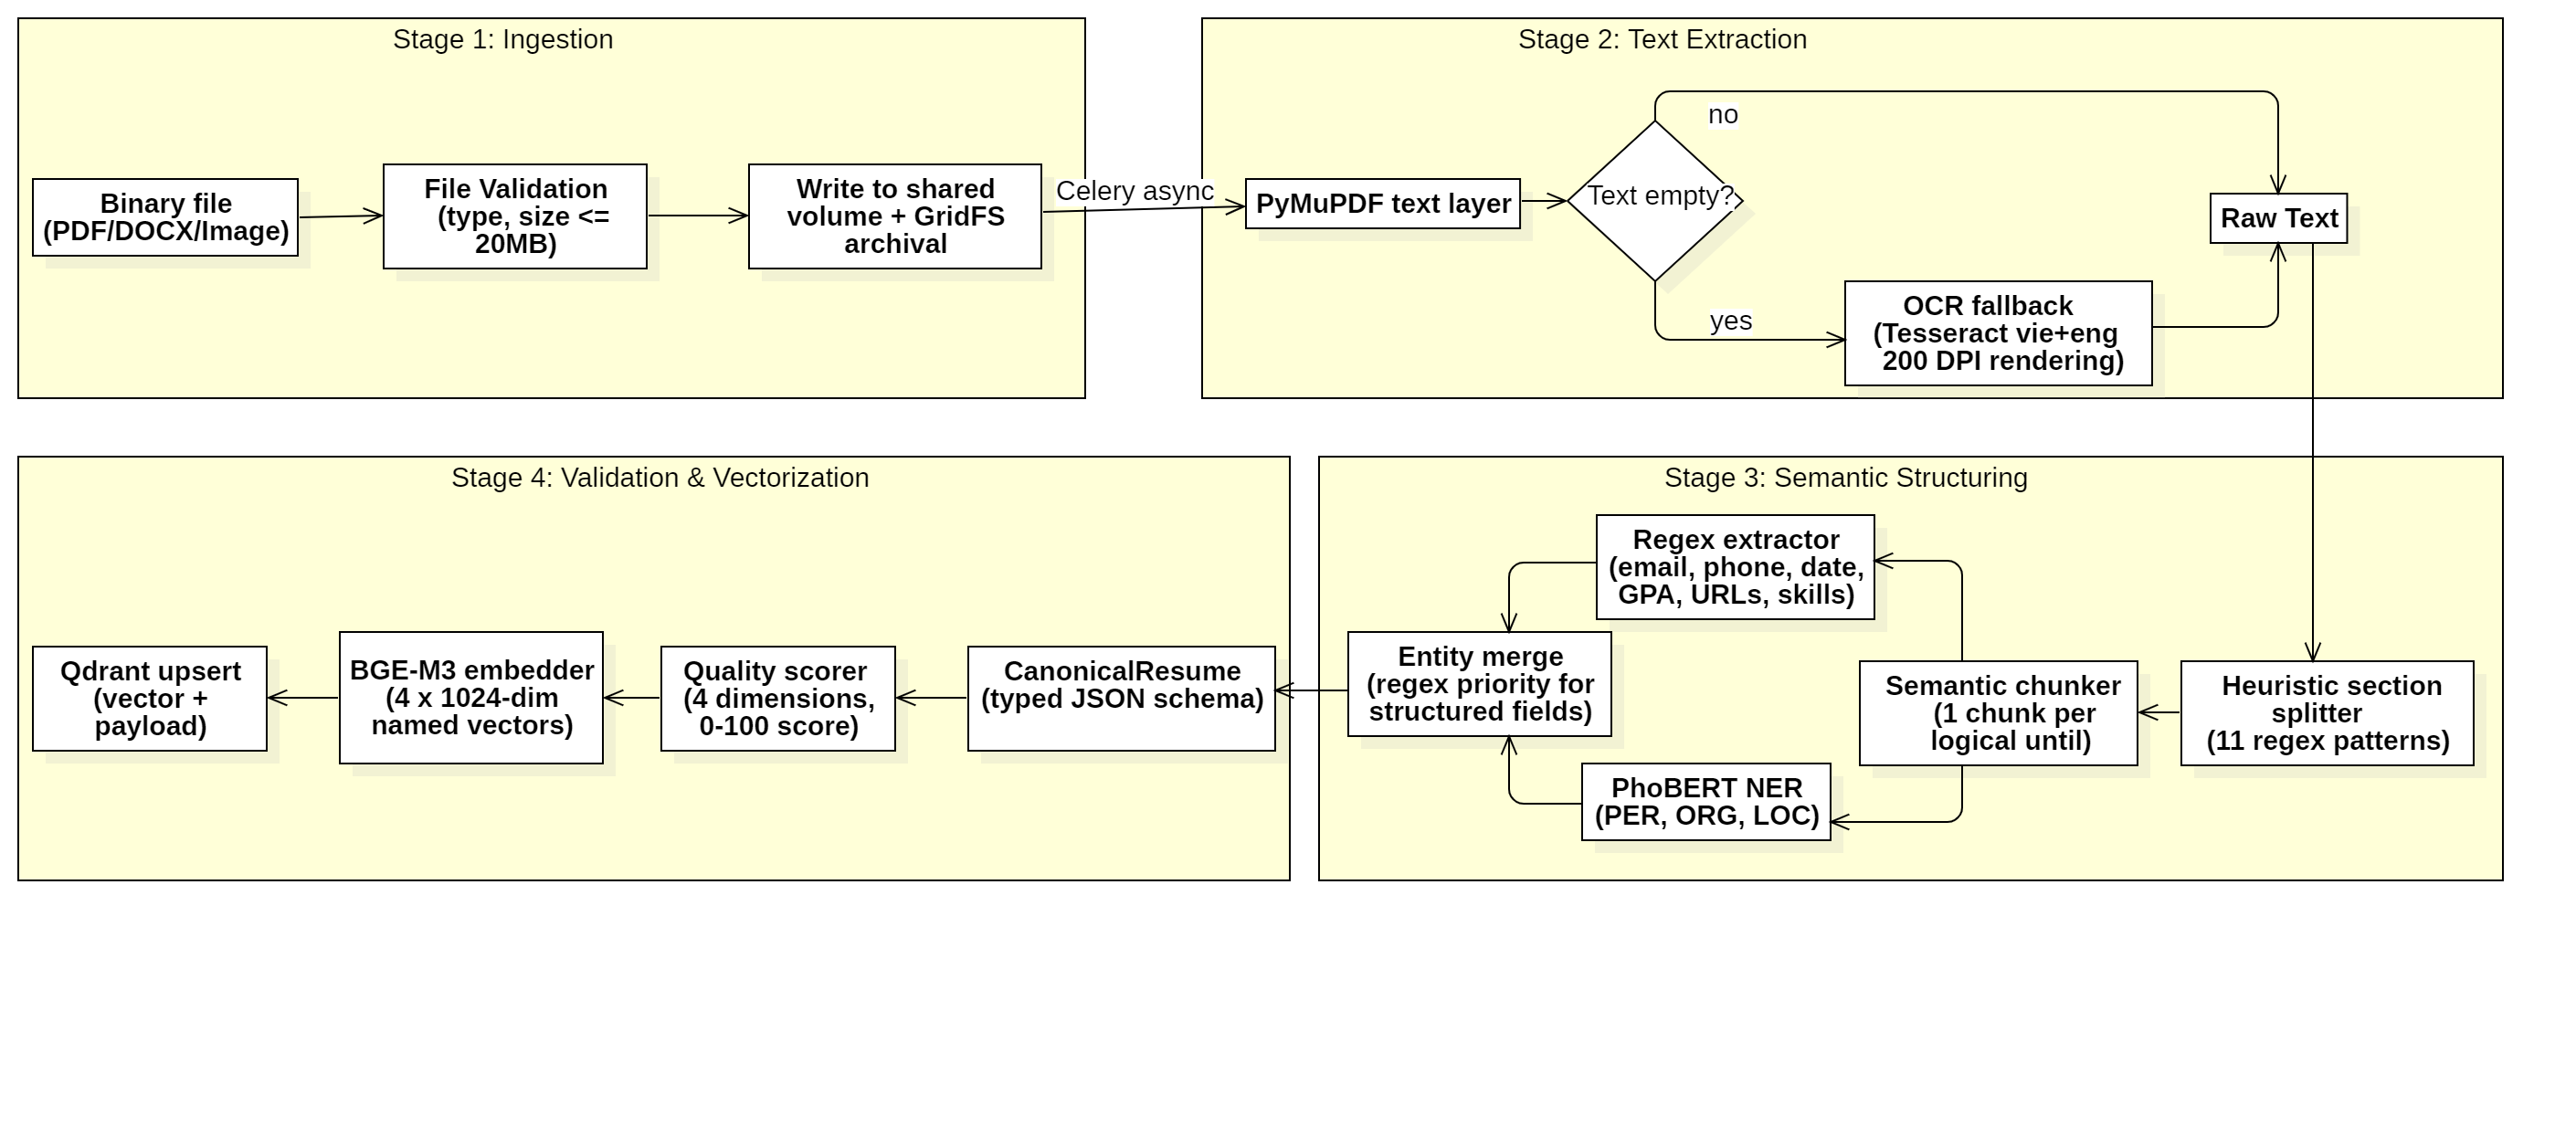
\includegraphics[width=0.85\textwidth]{thesis_1_images/chapter_1_thesis_1_diagram_5.png}
    \caption[End-to-end CV upload pipeline flowchart]{\textbf{End-to-end CV upload pipeline flowchart}: \textmd{Raw documents are converted, chunked, normalized, scored, and indexed asynchronously.}}
\end{figure}

The pipeline transforms data through four increasingly structured representations:

\begin{table}[H]
    \centering
    \caption[CV Processing Stages]{\textbf{CV Processing Stages}}
    \vspace{0.2cm}
    \normalsize
    \renewcommand{\arraystretch}{1.3}
    \begin{tabularx}{\textwidth}{Z{0.6} | Z{1.0} | Z{1.0} | Z{1.4}}
    \hline\hline
    Stage & Input & Output & Transformation \\
    \hline
    \textbf{Ingestion} & Binary file (PDF/DOCX/Image) & Raw bytes on shared volume & Format validation, zero-copy exchange \\
    \textbf{Text Extraction} & Raw bytes & Unstructured text string & PyMuPDF parsing or Tesseract OCR fallback \\
    \textbf{Semantic Structuring} & Flat text & \texttt{CanonicalResume} typed JSON & Section splitting $\rightarrow$ chunking $\rightarrow$ entity extraction $\rightarrow$ merge \\
    \textbf{Validation \& Vectorization} & Typed JSON & Quality-scored vectors in Qdrant & Multi-criteria scoring + BGE-M3 dense embeddings \\
    \hline\hline
    \end{tabularx}
\end{table}

Each stage progressively adds structure and semantic meaning to the data. The unstructured binary input gains textual form through parsing, textual form gains semantic labels through entity extraction, and labeled entities gain mathematical representations through vectorization - culminating in a rich, searchable resume representation that downstream tools (CV assessment, job matching, interview preparation) can consume directly.

This same four-stage pipeline serves dual purposes: at training time, it processes synthetic CVs to build the training dataset; at inference time, it processes real user uploads to populate the vector database. The architectural reuse ensures consistency between the data representations the model was trained on and those it encounters at runtime.

\vspace{0.8cm}
\addcontentsline{toc}{section}{3.2 Polyglot Persistence Architecture}
\noindent{\LARGE \textbf{3.2 Polyglot Persistence Architecture}\par}
\vspace{0.4cm}

\addcontentsline{toc}{subsection}{3.2.1 Overview}
\noindent{\Large \textbf{3.2.1 Overview}\par}
\vspace{0.4cm}

The AI chatbot operates across four distinct data access patterns that no single database can serve optimally: sub-millisecond reads of active session state, flexible document queries over unstructured conversation history, high-dimensional similarity search across vectorized resumes, and relational integrity for persistent user profiles with row-level tenant isolation. Rather than forcing these patterns into a single storage engine - accepting poor performance in at least three of the four - the system adopts a polyglot persistence strategy: each database is selected for the access pattern it was designed to optimize.

This chapter presents the architectural rationale behind the four-database topology, the data flows that connect them, and the design tradeoffs that govern their interaction. The focus is on three cross-cutting concerns: how session data moves through a lifecycle of creation, hydration, eviction, and restoration across database boundaries; how conversation state transforms from individual messages into a managed context window with extractive summarization; and how resume data flows from raw binary uploads through increasingly structured representations until it reaches a vector-searchable form.

Redis provides the in-memory session cache - the first tier that every read request hits before falling through to slower, more durable stores. MongoDB serves as the durable document store for conversation history, session metadata, and raw binary files via GridFS, providing the source-of-truth that outlives Redis TTL eviction. Qdrant stores dense vector embeddings that enable semantic search and skill-gap analysis, capabilities that neither Redis nor MongoDB can provide. Supabase (PostgreSQL) provides the persistent, user-scoped storage layer with relational integrity and database-level access control, ensuring that resume data survives across chatbot sessions and that tenant isolation is enforced independently of application logic.

\vspace{0.6cm}
\addcontentsline{toc}{subsection}{3.2.2 Session Lifecycle Pipeline}
\noindent{\Large \textbf{3.2.2 Session Lifecycle Pipeline}\par}
\vspace{0.4cm}

A chatbot session passes through five distinct states as it moves across the persistence layer. Understanding this lifecycle is essential to understanding why the system writes the same data to two databases simultaneously and why it maintains a three-tier fallback chain for reads.

\begin{figure}[H]
    \centering
    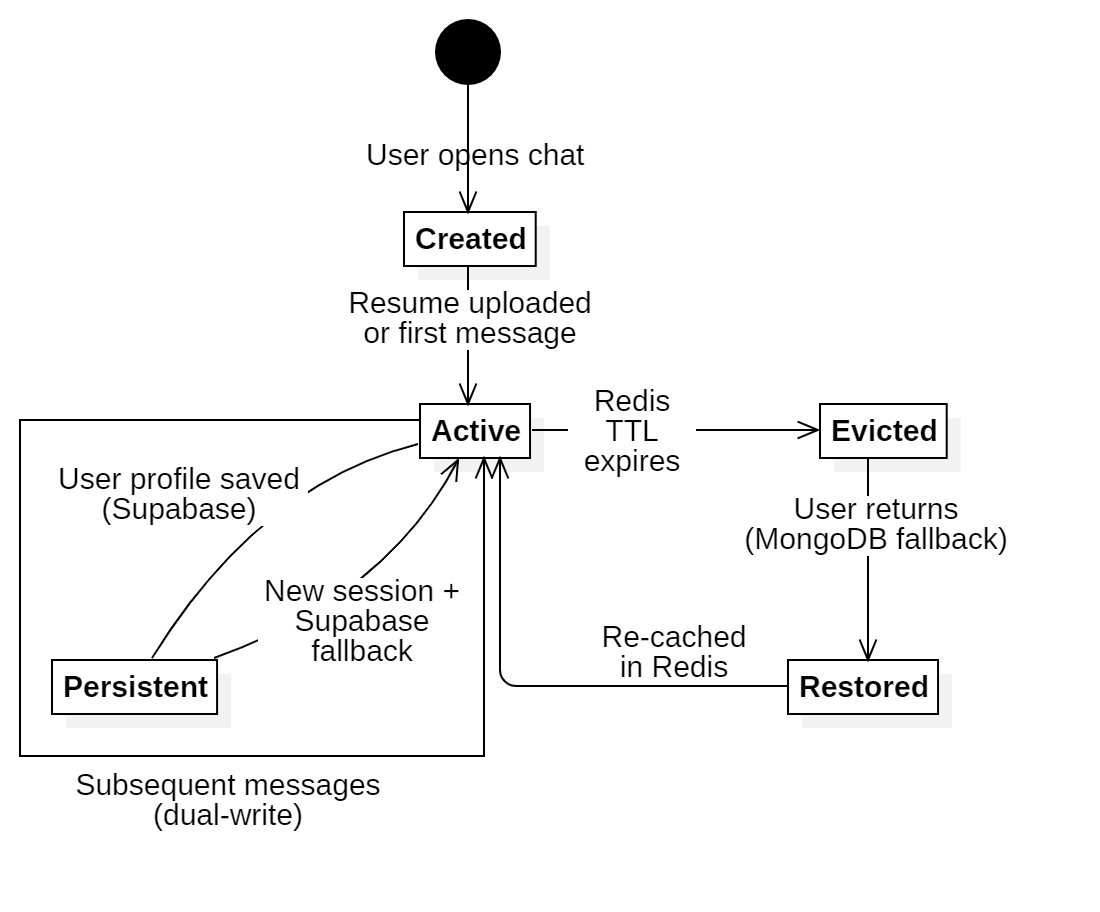
\includegraphics[width=0.85\textwidth]{thesis_1_images/chapter_3_thesis_1_diagram_1.png}
    \caption[Session lifecycle state diagram]{\textbf{Session lifecycle state diagram}: \textmd{Represents creation, active usage, dual-write synchronization, eviction, and restoration states.}}
\end{figure}

Created $\rightarrow$ Active: When a user initiates a conversation or uploads a resume, the system creates a session entry in Redis with a 24-hour time-to-live. If a resume is attached, the parsed JSON is bound to the session alongside the Qdrant vector identifier and the original filename. This initial write also propagates to MongoDB through an upsert operation, establishing the durable copy that will outlive the cache.

Active $\rightarrow$ Active (Dual-Write): Every session update - new resume binding, conversation turn, context summary - writes to both Redis and MongoDB in sequence. Redis provides the sub-millisecond read latency required for real-time chat interactions; MongoDB provides the durability guarantee that survives cache eviction and service restarts. The system prioritizes write consistency over write performance: both writes must succeed before the operation returns, ensuring the durable store never lags behind the cache.

Active $\rightarrow$ Evicted $\rightarrow$ Restored: When a session's 24-hour TTL expires in Redis, the data is silently evicted. If the user returns, the system detects the cache miss and transparently falls through to MongoDB, retrieves the session data, re-caches it in Redis with a fresh TTL, and resumes the conversation as though no interruption occurred. This fallback is invisible to the user and to the upstream chat endpoint - the session store abstracts the recovery behind a single read interface.

Active $\rightarrow$ Persistent: For authenticated users, resume data is additionally persisted to Supabase (PostgreSQL), creating a user-scoped record that survives not just cache eviction but session expiration entirely. This enables the third fallback tier: when a returning user starts a new chatbot session, the system checks Supabase for previously analyzed resume data and injects it into the new session context, eliminating the need for re-upload.

The three-tier fallback chain - Redis $\rightarrow$ MongoDB $\rightarrow$ Supabase - reflects a deliberate architectural ordering from fastest-but-ephemeral to slowest-but-permanent. Each tier serves a different temporal scope: Redis holds active sessions (minutes to hours), MongoDB holds session history (days to weeks), and Supabase holds user profiles (indefinitely).

\begin{figure}[H]
    \centering
    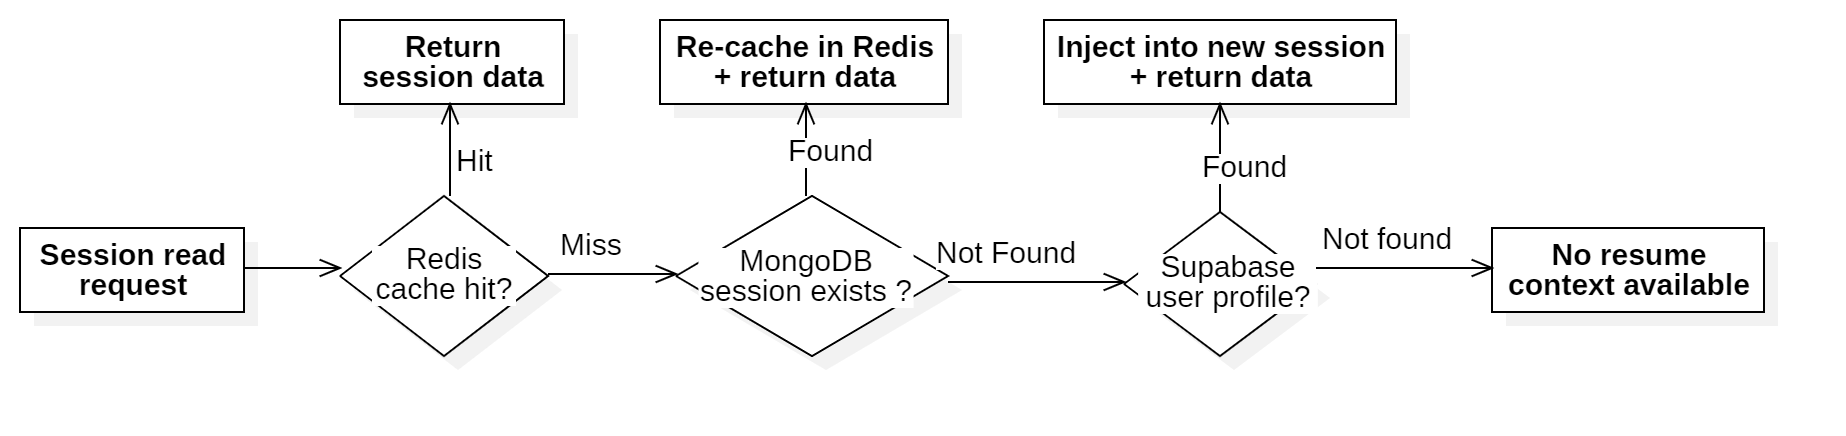
\includegraphics[width=0.85\textwidth]{thesis_1_images/chapter_3_thesis_1_diagram_2.png}
    \caption[Three-tier session read fallback chain]{\textbf{Three-tier session read fallback chain}: \textmd{The chatbot queries Redis, MongoDB, and Supabase sequentially to recover CV context.}}
\end{figure}

\vspace{0.6cm}
\addcontentsline{toc}{subsection}{3.2.3 Conversation State Machine}
\noindent{\Large \textbf{3.2.3 Conversation State Machine}\par}
\vspace{0.4cm}

Conversation data undergoes a series of transformations as it moves through the persistence layer, progressing from individual user messages into a managed context window that fits within the small language model's token budget. This transformation pipeline is central to the system's ability to maintain coherent multi-turn conversations despite the base model's limited context capacity.

\begin{figure}[H]
    \centering
    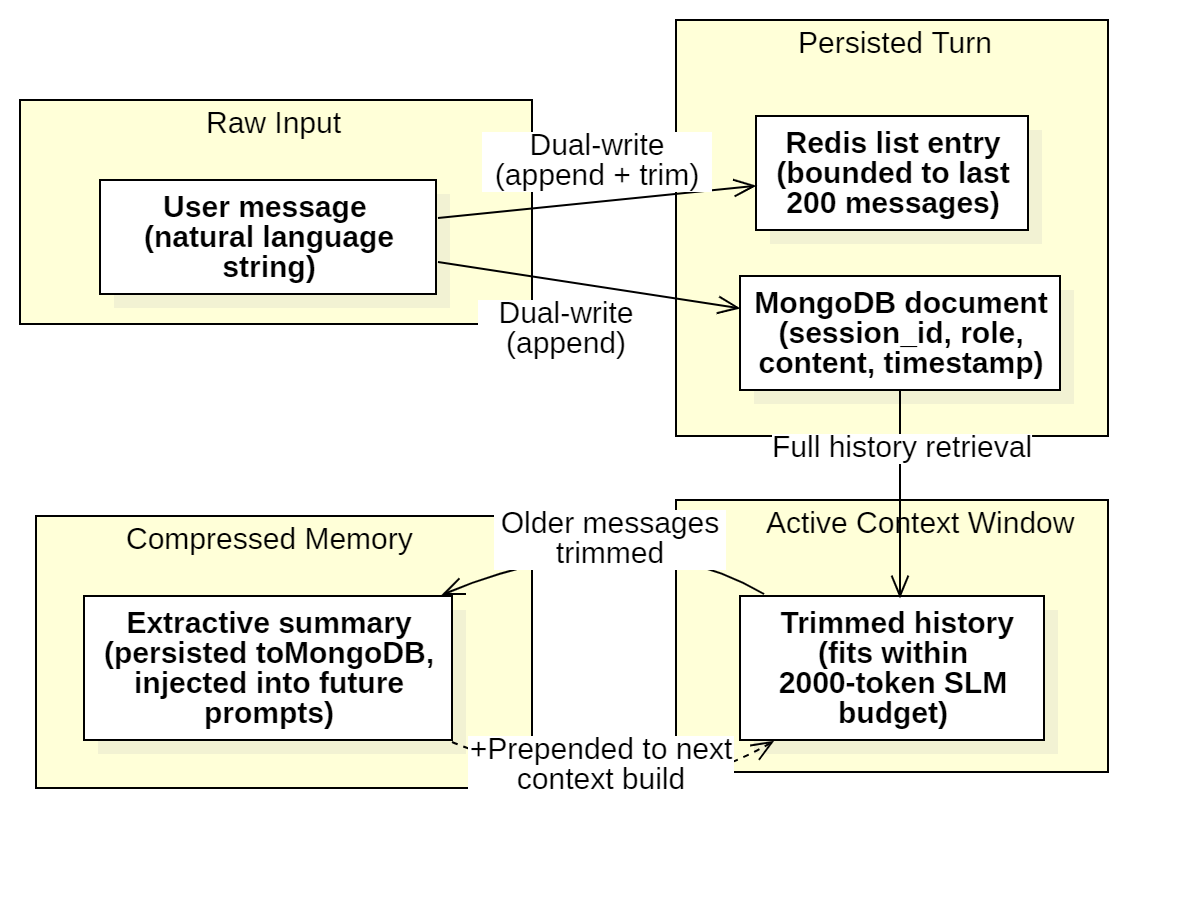
\includegraphics[width=0.85\textwidth]{thesis_1_images/chapter_3_thesis_1_diagram_3.png}
    \caption[Conversation state machine flowchart]{\textbf{Conversation state machine flowchart}: \textmd{Message history is serialized in Redis and archived in MongoDB to enforce a strict token sliding window.}}
\end{figure}

Raw Input $\rightarrow$ Persisted Turn: Each user or assistant message is appended to both MongoDB (as an individual document with session linkage and chronological timestamp) and Redis (as a serialized entry in a bounded list). The MongoDB copy is the source-of-truth: it retains the complete conversation history without length constraints. The Redis copy is a performance optimization: it caches the most recent turns for fast retrieval during active conversations, automatically discarding older entries to prevent unbounded memory growth.

The MongoDB collection uses a compound index on session identifier and timestamp, enabling chronologically ordered retrieval of an entire conversation thread through a single index scan. This index design eliminates the need for a sort operation at query time - the storage layer returns messages in the order they were spoken.

Persisted Turn $\rightarrow$ Active Context Window: When the chat endpoint prepares a prompt for the language model, it retrieves the full conversation history from MongoDB and passes it through the Context Window Manager. The manager evaluates the total token count against the model's 2,000-token budget and trims older messages from the beginning of the history until the remaining turns fit within the budget.

Active Context Window $\rightarrow$ Compressed Memory: When messages are trimmed, they are not simply discarded. The Context Window Manager generates an extractive summary of the dropped messages - a compressed representation that preserves the key topics, decisions, and user preferences from earlier in the conversation. This summary is persisted to MongoDB and prepended to the context window on subsequent requests, giving the model awareness of conversational history that has been evicted from the active window.

This summary-and-reinject pattern is the architectural answer to a fundamental constraint: the SLM's limited context window cannot hold long conversations, but users expect conversational continuity across dozens of turns. Rather than truncating silently (losing context) or paginating (adding complexity), the system compresses old context into a summary that occupies a fraction of the original token count while preserving the information most relevant to ongoing dialogue.

\vspace{0.6cm}
\addcontentsline{toc}{subsection}{3.2.4 Resume Data Pipeline}
\noindent{\Large \textbf{3.2.4 Resume Data Pipeline}\par}
\vspace{0.4cm}

Resume data follows the most complex cross-database flow in the system, touching all four databases as it transforms from an unstructured binary file into a searchable, AI-ready vector representation.

\begin{figure}[H]
    \centering
    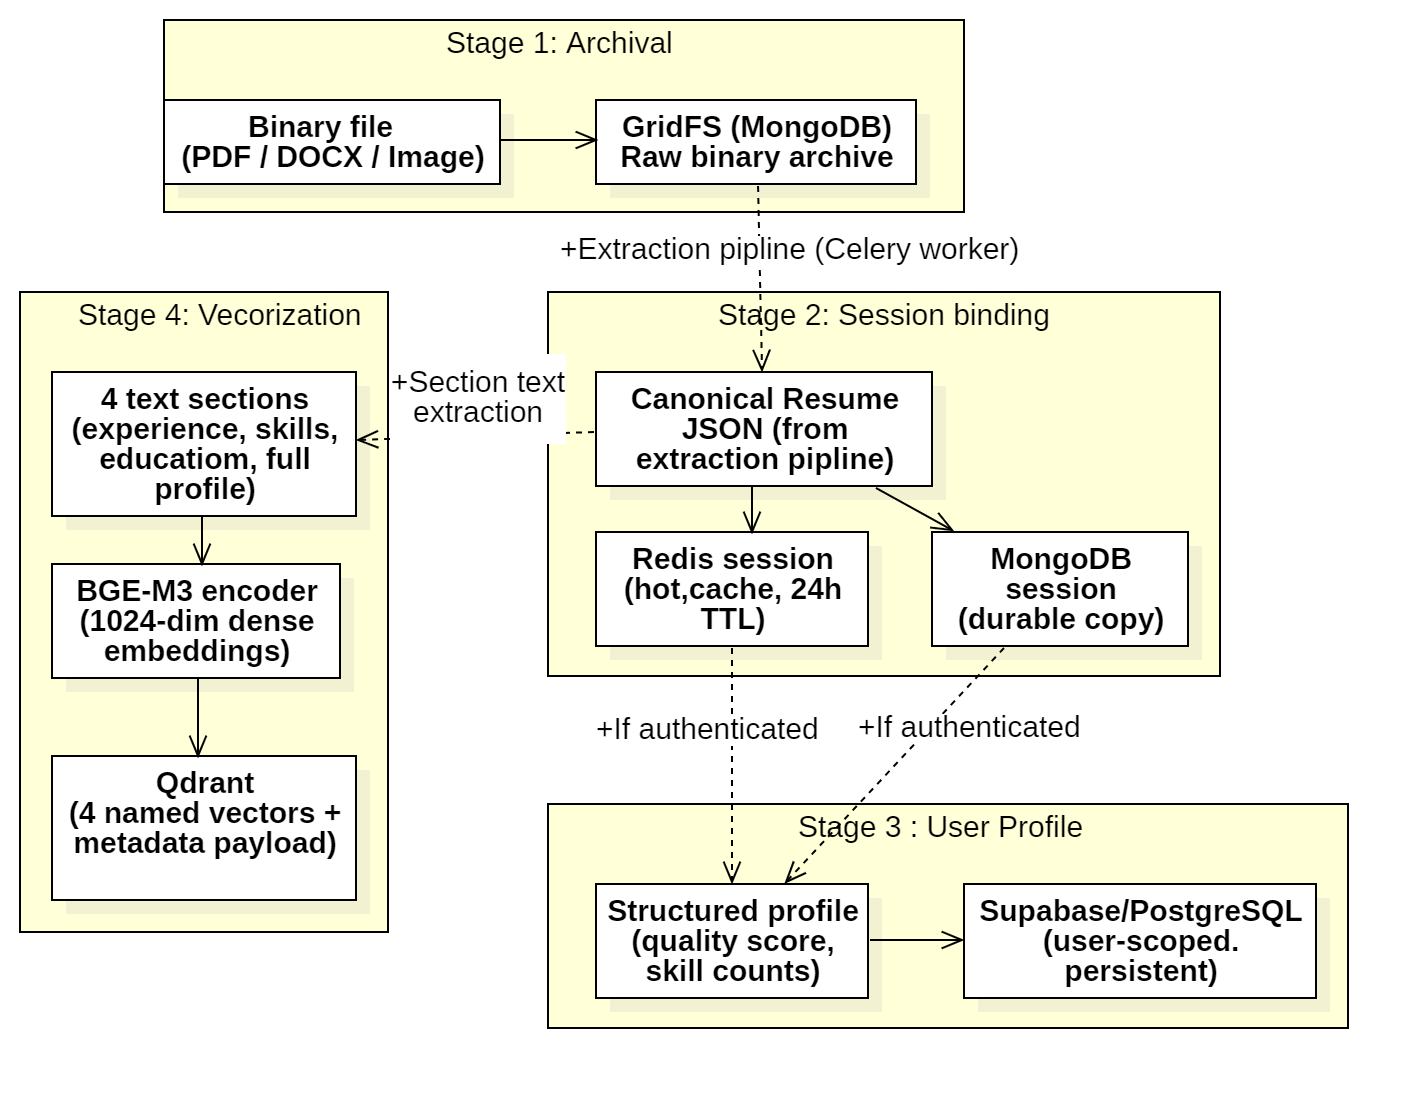
\includegraphics[width=0.85\textwidth]{thesis_1_images/chapter_3_thesis_1_diagram_4.png}
    \caption[Resume cross-database data pipeline]{\textbf{Resume cross-database data pipeline}: \textmd{Conversion logs are parsed, quality-scored, and saved to Qdrant (vectors) and MongoDB (documents).}}
\end{figure}

Archival (MongoDB GridFS): The raw binary file is archived in MongoDB's GridFS immediately upon upload, before any processing begins. This archival serves two purposes: it provides an immutable record of the original document for audit and re-extraction, and it decouples the binary storage concern from the extraction pipeline - if extraction fails or needs to be re-run with improved algorithms, the original file is always available without requiring the user to upload again.

Session Binding (Redis + MongoDB): Once the extraction pipeline produces a canonical resume JSON, the Celery worker binds it to the user's active session through the dual-write pattern described in §3.2.2. The resume JSON, the Qdrant vector identifier, and the original filename are written to both Redis and MongoDB, making the parsed resume immediately available to subsequent chat interactions. This binding is what enables the chatbot's resume-aware tools - CV assessment, job matching, interview preparation - to access the user's parsed profile without re-extraction.

User Profile (Supabase): For authenticated users, the structured profile data - including the canonical resume JSON, quality score, and aggregate metrics (skill count, experience count) - is persisted to Supabase. This write is the bridge between session-scoped and user-scoped persistence: the session may expire, but the user profile endures. The data stored here is the same canonical JSON produced by the extraction pipeline, but associated with the user's identity rather than a transient session identifier.

Vectorization (Qdrant): The extraction pipeline simultaneously generates four dense vector embeddings from different sections of the resume text, each encoding a different aspect of the candidate's profile. These vectors are stored as a single Qdrant point with four named vectors, enabling aspect-specific similarity search - a query against the skills vector returns resumes with similar skill profiles, while a query against the full profile vector returns holistically similar candidates.

The multi-vector architecture is a deliberate design choice that trades storage space (4$\times$ the vectors of a single-embedding approach) for retrieval precision. The chatbot's downstream tools exploit this granularity: job matching queries the skills vector for skill-gap analysis, while general resume search uses the full profile vector for holistic comparison. Each vector is accompanied by a metadata payload containing the candidate's structured attributes (seniority level, quality score, skill list), enabling filtered retrieval without secondary database lookups - the vector database serves as both the similarity engine and the metadata store for resume-aware operations.

\vspace{0.6cm}
\addcontentsline{toc}{subsection}{3.2.5 Tenant Isolation Architecture}
\noindent{\Large \textbf{3.2.5 Tenant Isolation Architecture}\par}
\vspace{0.4cm}

The system enforces data isolation at two architectural levels: database-level policies that are evaluated on every query regardless of application logic, and application-level ownership filters that restrict operations to the requesting user's data.

Database-Level Isolation (Supabase): The persistent user profile table enforces Row Level Security (RLS) policies directly in PostgreSQL, ensuring that every SELECT, INSERT, UPDATE, and DELETE operation is automatically filtered to the authenticated user's records. These policies are evaluated by the database engine itself - even a direct SQL query bypassing the application layer cannot access another user's data. The policies extract the authenticated user's identity from the JWT token and compare it against the ownership column on every row access.

The chatbot's backend service requires an exception to this isolation: the Celery worker performs server-side writes on behalf of users during asynchronous CV extraction, a context where no user JWT is available. This is resolved through a trust boundary decision - the worker connects with an elevated service-role key that bypasses RLS, while all user-facing endpoints connect with the user's scoped JWT. This bifurcation ensures that the least-privilege principle is maintained: user-facing code can never exceed the user's own data scope, while background workers operate under explicit, auditable elevated privileges.

Application-Level Isolation (MongoDB): The conversation management layer enforces ownership isolation through query-level filtering - every read, update, and delete operation includes the user's identity as a mandatory filter predicate. This provides defense-in-depth: even if a user somehow obtains another user's conversation identifier, the query filter prevents cross-tenant access. MongoDB does not natively support row-level security policies comparable to PostgreSQL's, making this application-level enforcement the primary isolation mechanism for conversation data.

\vspace{0.6cm}
\addcontentsline{toc}{subsection}{3.2.6 Design Tradeoffs}
\noindent{\Large \textbf{3.2.6 Design Tradeoffs}\par}
\vspace{0.4cm}

\noindent{\large \textbf{3.2.6.1 Four Databases vs. One}\par}
\vspace{0.3cm}

The polyglot persistence strategy introduces operational complexity: four databases to deploy, monitor, back up, and maintain, each with its own failure mode and scaling characteristics. The alternative - consolidating into PostgreSQL (which can serve as a cache via \texttt{UNLOGGED} tables, a document store via JSONB, and a vector store via pgvector) - would simplify operations at the cost of performance in at least two access patterns. Redis outperforms PostgreSQL for session reads by an order of magnitude, and Qdrant's HNSW index provides sub-100ms approximate nearest-neighbor search at a scale where pgvector's exact search degrades significantly. The system accepts the operational cost because the chatbot's real-time responsiveness depends on each database operating within its designed performance envelope.

\noindent{\large \textbf{3.2.6.2 Dual-Write vs. Event Sourcing}\par}
\vspace{0.3cm}

The dual-write pattern (writing to both Redis and MongoDB in the same request path) introduces a consistency risk: if the MongoDB write fails after the Redis write succeeds, the cache contains data that the durable store does not. An event-sourcing architecture - where all state changes are appended to an immutable event log and materialized views are derived from replay - would eliminate this risk but add significant architectural complexity for a system where the failure mode is benign: a missed MongoDB write means the session cannot be restored after Redis eviction, but no data is corrupted. The system accepts this risk because session data is inherently ephemeral and can be regenerated by re-uploading a resume.

\noindent{\large \textbf{3.2.6.3 Embedded Messages vs. Referenced Documents}\par}
\vspace{0.3cm}

Conversation messages in the sidebar's persistence layer are embedded as an array within the conversation document rather than stored as individual referenced documents. This trades write amplification (every new message rewrites the parent document's array) for read atomicity (loading a conversation retrieves the complete thread in a single query without joins). For a chatbot where conversations rarely exceed a few hundred messages, the document size remains well within MongoDB's 16 MB limit, and the read performance benefit - a single round-trip instead of a join across two collections - directly impacts the sidebar's perceived responsiveness when switching between conversations.

\vspace{0.8cm}
\addcontentsline{toc}{section}{3.3 Frontend AI Presentation Layer}
\noindent{\LARGE \textbf{3.3 Frontend AI Presentation Layer}\par}
\vspace{0.4cm}

\addcontentsline{toc}{subsection}{3.3.1 Overview}
\noindent{\Large \textbf{3.3.1 Overview}\par}
\vspace{0.4cm}

The frontend presentation layer serves as the user-facing coordination surface for the CareerIntel platform, bridging the interface with the synchronous inference and asynchronous processing domains (introduced in \S3.1.2). Built on the Next.js App Router paradigm, the presentation layer translates user interactions into API orchestration calls while managing state reactivity, asynchronous machine learning tasks, and conversation history.

This section details the frontend orchestration architecture. It describes how the server-client rendering boundary isolates backend credentials while maintaining a responsive UI; how the asynchronous task pipeline handles file uploads, polling coordination, and backend failure mitigation; how conversation state integrates with the polyglot persistence layer; and how the presentation layer routes and renders responses based on upstream AI adapters. The section concludes with an analysis of the core architectural tradeoffs governing the presentation layer's design.

\vspace{0.6cm}
\addcontentsline{toc}{subsection}{3.3.2 Server-Client Rendering Boundary}
\noindent{\Large \textbf{3.3.2 Server-Client Rendering Boundary}\par}
\vspace{0.4cm}

The presentation layer utilizes the Next.js App Router to separate server-side data fetching and authentication from client-side UI reactivity. Rather than mixing credential management with UI execution, the architecture enforces a strict Trust Boundary Pattern that dictates where application logic is executed.

\begin{figure}[H]
    \centering
    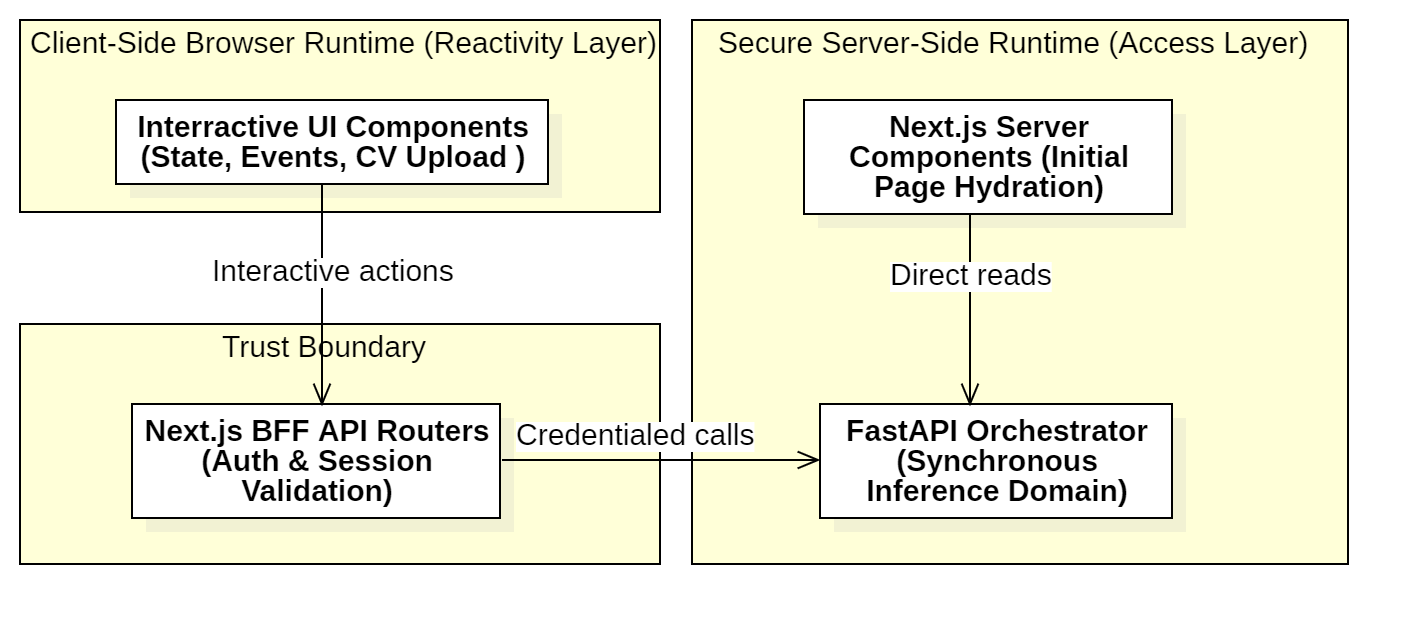
\includegraphics[width=0.85\textwidth]{thesis_1_images/chapter_6_thesis_1_diagram_1.png}
    \caption[Server-client rendering trust boundary]{\textbf{Server-client rendering trust boundary}: \textmd{Secure server components fetch initial page content, client components manage micro-interactions, and BFF routes proxy backend requests.}}
\end{figure}

\noindent{\large \textbf{3.3.2.1 Secure Server Components}\par}
\vspace{0.3cm}

The entry point for the conversational interface (\texttt{/ai}) runs exclusively within the secure server runtime. Server Components manage:
\begin{itemize}
    \item Credential Isolation: Performing tenant authentication and session verification without exposing database connection strings, security tokens, or environment keys to the browser.
    \item Initial Hydration: Querying the FastAPI orchestrator directly during page generation to retrieve the user's active session metadata and recent conversation list. This eliminates the latency of a secondary client-side API round-trip during the initial load.
\end{itemize}

\noindent{\large \textbf{3.3.2.2 Reactive Client Components}\par}
\vspace{0.3cm}

The interactive chat elements operate inside the client-side browser runtime, separated by the \texttt{"use client"} declaration boundary. Client Components handle:
\begin{itemize}
    \item Interactive State: Maintaining the local message feed, capture of file-upload payloads, and dynamic sidebar updates in response to user inputs.
    \item Micro-interactions: Orchestrating local layout adjustments, typing indicators, and user-initiated actions that require immediate response without server latency.
\end{itemize}

\vspace{0.6cm}
\addcontentsline{toc}{subsection}{3.3.3 Asynchronous Task Coordination Pipeline}
\noindent{\Large \textbf{3.3.3 Asynchronous Task Coordination Pipeline}\par}
\vspace{0.4cm}

Processing unstructured resumes involves computationally heavy tasks (such as parsing, Named Entity Recognition, and embedding generation) that exceed standard HTTP timeout limits. To keep the UI responsive, the presentation layer orchestrates uploads and status checks through a decoupled, asynchronous pipeline mediated by a Backend-For-Frontend (BFF) proxy.

\begin{figure}[H]
    \centering
    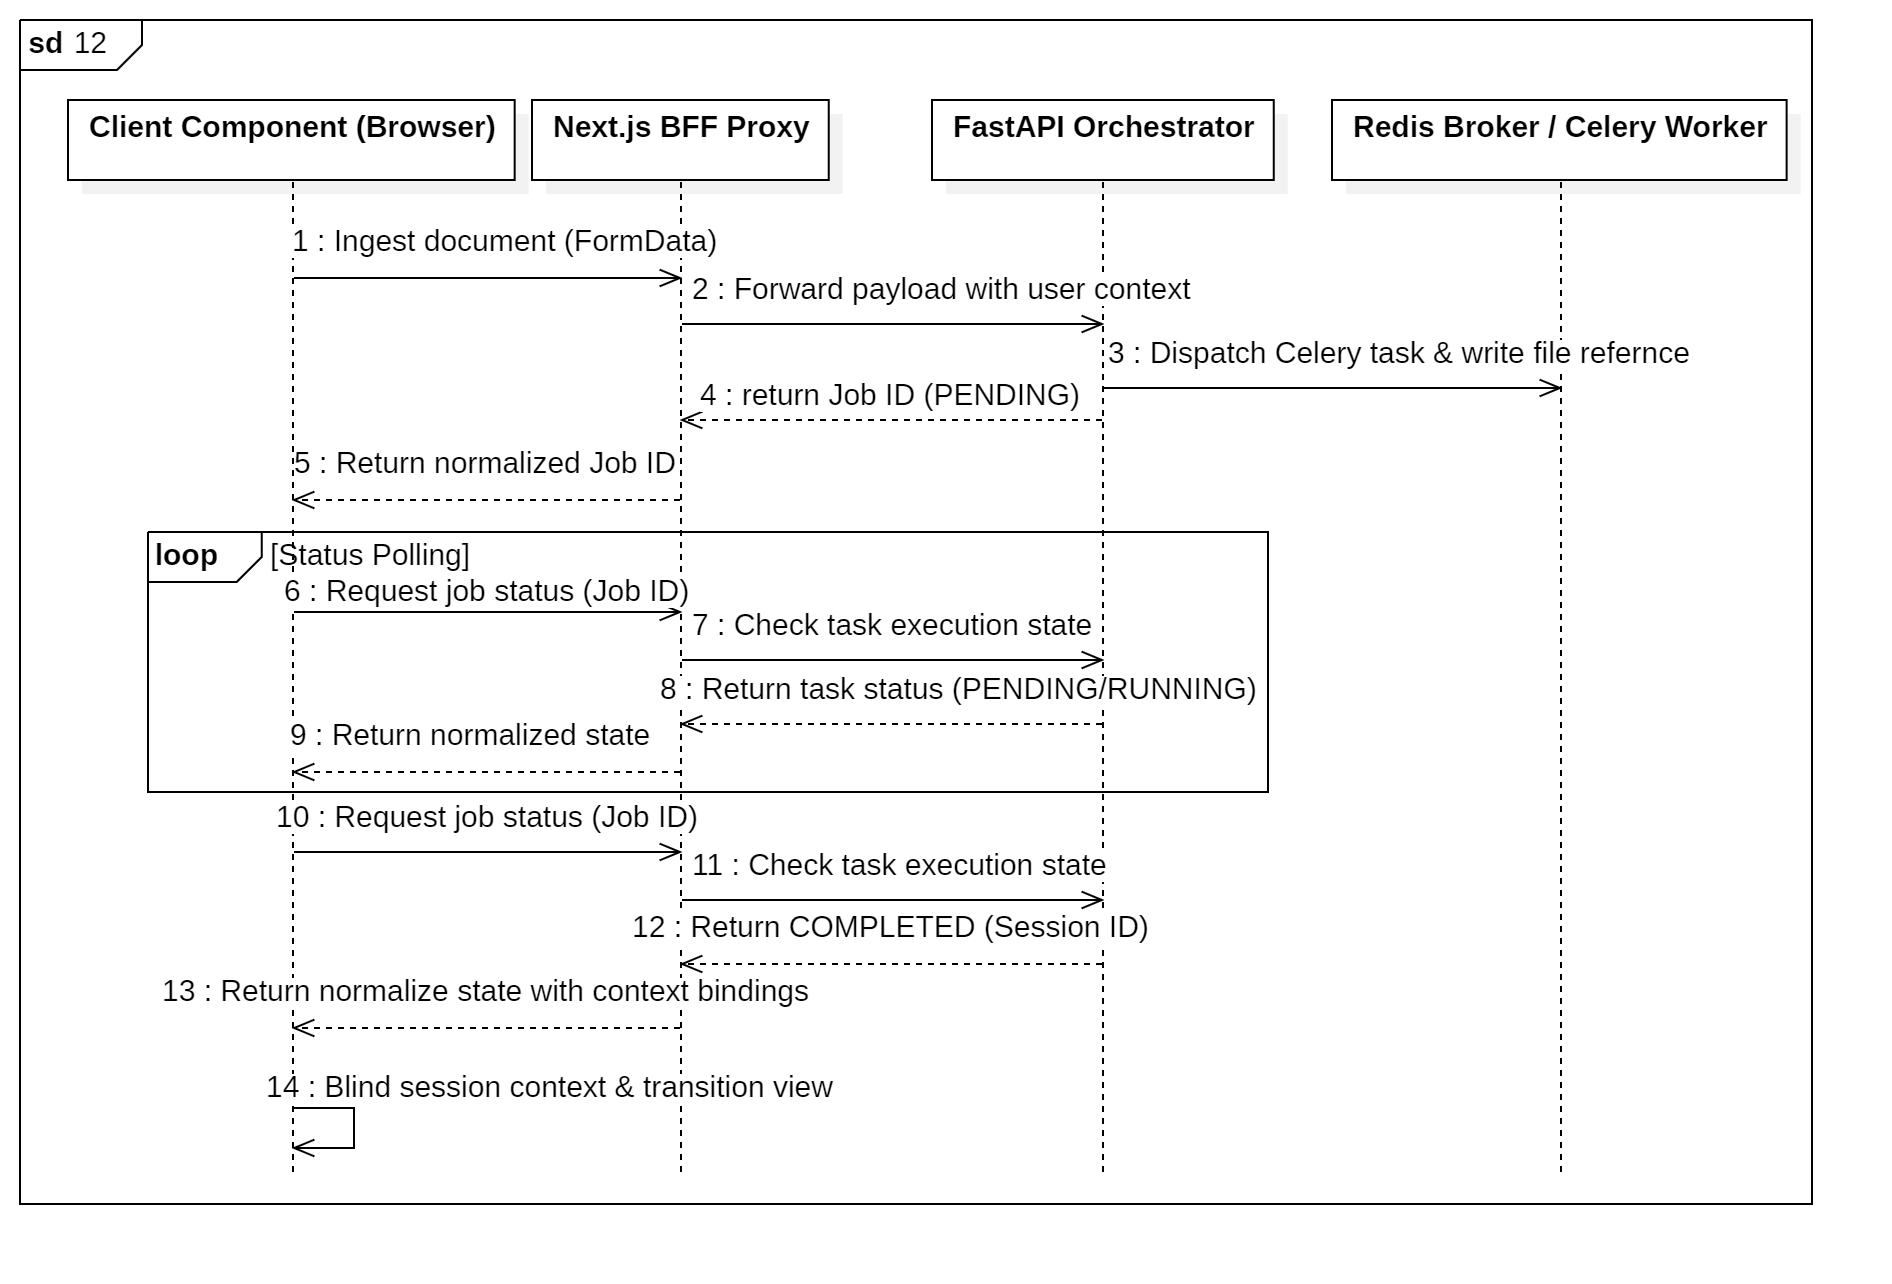
\includegraphics[width=0.85\textwidth]{thesis_1_images/chapter_6_thesis_1_diagram_2.png}
    \caption[Asynchronous task coordination sequence diagram]{\textbf{Asynchronous task coordination sequence diagram}: \textmd{The client uploads files asynchronously and polls backend job endpoints to track extraction progress.}}
\end{figure}

\noindent{\large \textbf{3.3.3.1 Ingestion and Task Dispatch}\par}
\vspace{0.3cm}

When a user attaches a CV, the presentation layer captures the file, runs initial type checks, and transmits the payload to the BFF upload proxy. The BFF forwards the request to the FastAPI orchestrator, which archives the raw document in MongoDB GridFS, writes the file to the shared volume, and dispatches a background processing task to the Redis-backed Celery worker (as described in §3.1.4.2). The API immediately returns a unique job identifier, freeing the client from waiting for the extraction process to complete.

\noindent{\large \textbf{3.3.3.2 Status Polling and Progress Tracking}\par}
\vspace{0.3cm}

Upon receiving the job identifier, the client UI transitions to a processing state and enters a polling loop. The client queries the BFF status endpoint at regular intervals to trace task execution. If the task remains active, the UI displays dynamic progress updates to manage user expectations. If the task fails or times out, the client handles the transition gracefully, allowing the user to retry without losing conversation state.

\noindent{\large \textbf{3.3.3.3 BFF Error Normalization Boundary}\par}
\vspace{0.3cm}

The Next.js API routes act as an Error Normalization Boundary between the frontend and the upstream AI services. If the FastAPI backend encounters a database timeout, an out-of-memory error during inference, or is temporarily unreachable, the BFF intercepts these raw failures. Instead of exposing raw stack traces or throwing unhandled exceptions that could crash the React UI, the BFF normalizes these responses into a standard JSON error payload. This structure allows the client component to transition to a controlled error state and offer context-specific recovery paths.

\vspace{0.6cm}
\addcontentsline{toc}{subsection}{3.3.4 Conversation State Architecture}
\noindent{\Large \textbf{3.3.4 Conversation State Architecture}\par}
\vspace{0.4cm}

The conversational sidebar manages active session states, historical list retrieval, and session renaming or archiving. This layer interacts directly with the polyglot persistence architecture described in \S3.2.

\noindent{\large \textbf{3.3.4.1 Conversation Lifecycles}\par}
\vspace{0.3cm}

Conversation documents are persisted in MongoDB (as described in \S3.2.3). The presentation layer manages these states through server-side CRUD endpoints:
\begin{itemize}
    \item Title Generation: To eliminate manual title entry, the system automatically derives a thread title from the initial user turn, trimming it to fit the sidebar constraints.
    \item Soft Deletion: Archiving operations mark records as soft-deleted to keep the sidebar list clean while preserving historical records for potential restoration.
    \item Tenant Isolation: Every CRUD operation is verified at the BFF layer by cross-checking the requester's authenticated identifier against the record owner, preventing cross-tenant access.
\end{itemize}

\noindent{\large \textbf{3.3.4.2 Session Identity Linkage}\par}
\vspace{0.3cm}

When a conversation starts, it receives a client-side identity. If the user subsequently uploads a resume, the extraction pipeline binds the generated parsed context to a backend session ID (see §3.2.4). The presentation layer links these identifiers together. When a user switches between sidebar conversations, the client passes the linked backend session ID to the FastAPI orchestrator, allowing the backend to restore vector search parameters and retrieve CV embeddings from Qdrant without reprocessing the original document.

\vspace{0.6cm}
\addcontentsline{toc}{subsection}{3.3.5 Response Rendering Pipeline}
\noindent{\Large \textbf{3.3.5 Response Rendering Pipeline}\par}
\vspace{0.4cm}

The presentation layer uses a Presentation Router Pattern to handle structured outputs from the different backend AI adapters. The frontend acts as a template compiler, routing responses based on their declared type to ensure specialized data formats are rendered correctly.

\begin{figure}[H]
    \centering
    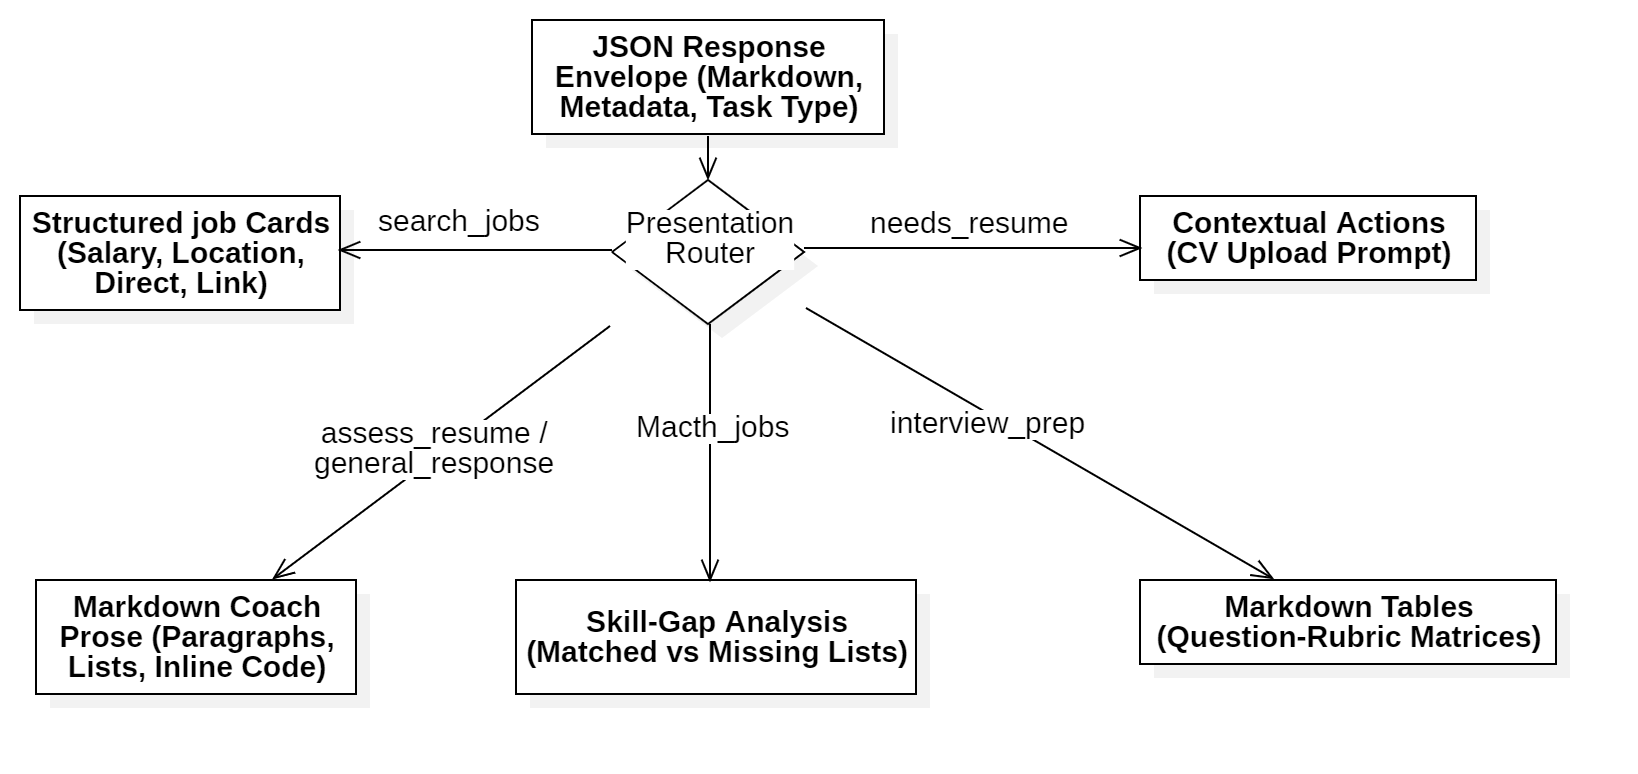
\includegraphics[width=0.85\textwidth]{thesis_1_images/chapter_6_thesis_1_diagram_3.png}
    \caption[Response presentation router]{\textbf{Response presentation router}: \textmd{The frontend dynamically switches its visual rendering layout based on the task type envelope returned by the backend API.}}
\end{figure}

\noindent{\large \textbf{3.3.5.1 Task-Type Presentation Routing}\par}
\vspace{0.3cm}

The backend returns a unified JSON response envelope containing the text payload, execution metadata, and a classification label (\texttt{task\_type}). The presentation layer parses this label and routes the payload to the appropriate UI layout:
\begin{itemize}
    \item Coaching and Conversations (\texttt{assess\_resume}, \texttt{general\_response}): Routed to the standard Markdown renderer, displaying paragraphs, bold highlights, lists, and inline code generated by Adapter B.
    \item Structured Preparation Matrices (\texttt{interview\_prep}): Formatted as multi-column Markdown tables that align interview questions, candidate evaluation rubrics, and recommended study paths generated by Adapter C.
    \item Job Search Listings (\texttt{search\_jobs}): Bypasses standard Markdown rendering. The UI compiles the raw search results from Elasticsearch into structured, interactive job cards containing salary badges, locations, and direct application links.
    \item Skill Gap Assessments (\texttt{match\_jobs}): Renders visual lists that compare candidate skills against job requirements, grouping them into matched and missing lists for easy scanning.
    \item Contextual Actions (\texttt{needs\_resume}): Renders helper prompts and action buttons (such as triggering the file attachment workflow) when a resume is required but has not yet been bound to the session.
\end{itemize}

\vspace{0.6cm}
\addcontentsline{toc}{subsection}{3.3.6 Design Tradeoffs}
\noindent{\Large \textbf{3.3.6 Design Tradeoffs}\par}
\vspace{0.4cm}

\noindent{\large \textbf{3.3.6.1 Asynchronous Long-Polling vs. WebSockets vs. SSE}\par}
\vspace{0.3cm}

The choice of client-polling over persistent connection protocols (such as WebSockets or Server-Sent Events) represents a trade of connection overhead for system simplicity:
\begin{itemize}
    \item WebSockets and SSE: Offer lower latency and real-time push capability, but they require persistent server connections. This complicates load balancing, increases memory consumption at the BFF layer under high concurrent loads, and requires complex client-side reconnection logic.
    \item Long-Polling: Operates over standard, stateless HTTP requests. It works out-of-the-box with serverless and edge infrastructure, integrates with standard authentication models, and avoids holding open long-lived sockets. Polling every two seconds introduces negligible network overhead for the relatively low frequency of CV uploads, while drastically simplifying the BFF deployment.
\end{itemize}

\noindent{\large \textbf{3.3.6.2 BFF Error Normalization vs. Upstream Proxying}\par}
\vspace{0.3cm}

The error normalization boundary adds development complexity but significantly increases frontend resilience:
\begin{itemize}
    \item Upstream Proxying: Directly forwarding raw backend responses reduces BFF code and simplifies debugging during development, but it exposes the client to raw framework errors, database tracebacks, or system timeouts.
    \item BFF Error Normalization: Intercepting and wrapping all upstream exceptions into standardized frontend states ensures the client UI never crashes due to unexpected backend failures. This trade prioritizes user-facing durability and graceful degradation over raw error visibility.
\end{itemize}

\noindent{\large \textbf{3.3.6.3 Embedded Messages vs. Client-Side State Management}\par}
\vspace{0.3cm}

Managing conversation state directly through server-side MongoDB reads (leveraging the embedded messages structure in §3.2.6.3) trades client-side flexibility for structural simplicity:
\begin{itemize}
    \item Client-Side State Management: Using complex global state containers allows for advanced offline editing and client-side filtering, but it increases code bundle sizes and introduces consistency issues when sync operations fail.
    \item Embedded Messages: Keeps the client state stateless. Clicking a conversation fetches the entire thread in a single, fast document query. The UI remains simple, reactivity is handled by React's local state, and the server retains the authoritative conversation history, ensuring a consistent user experience across multiple devices.
\end{itemize}

\vspace{0.8cm}
Having described how the frontend presentation layer consumes and renders AI-generated responses, we now turn to the backend orchestrator that produces them. The following section details the FastAPI-based coordination engine, its multi-adapter inference strategy, and the intent classification pipeline that routes user messages to specialized model adapters.

\vspace{0.4cm}
\addcontentsline{toc}{section}{3.4 AI Chatbot Orchestrator - SLM Multi-Adapter Architecture}
\noindent{\LARGE \textbf{3.4 AI Chatbot Orchestrator - SLM Multi-Adapter Architecture}\par}
\vspace{0.4cm}

\addcontentsline{toc}{subsection}{3.4.1 Overview}
\noindent{\Large \textbf{3.4.1 Overview}\par}
\vspace{0.4cm}

The AI chatbot orchestrator serves as the central coordination surface of the CareerIntel platform. It organizes real-time user interactions through a Multi-Adapter Small Language Model (SLM) architecture, in which three specialized adapters-fine-tuned via QLoRA-are mounted on a single shared Qwen2.5:1.5B base weights model. Rather than relying on outsourcing to massive monolithic models configured with varying system prompts, this architecture decomposes the user experience into task-specific sub-problems. This approach minimizes latency, ensures predictable output formatting, and fits within the memory constraints of consumer-grade hardware.

The orchestrator is structured around a FastAPI server that acts as a traffic router. It resolves session state, determines intent using Adapter A (intent classifier), and delegates execution to the Tool Dispatcher. The dispatcher routes requests to specialized search indices or downstream generation adapters: Adapter B (HR career coach) for natural Vietnamese prose, or Adapter C (structured content generator) for interview preparation matrices and roadmap tables.

\begin{figure}[H]
    \centering
    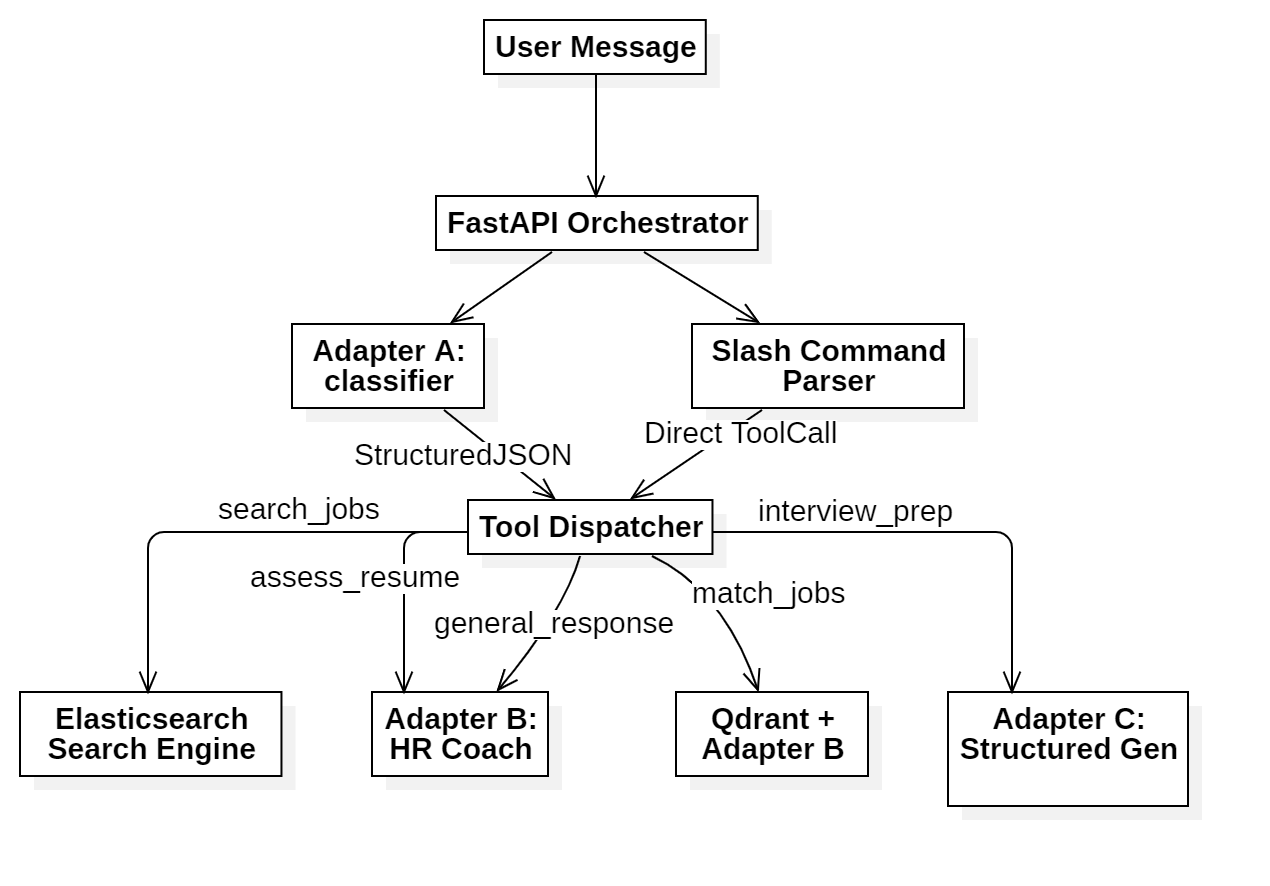
\includegraphics[width=0.85\textwidth]{thesis_1_images/chapter_7_thesis_1_diagram_1.png}
    \caption[Multi-adapter orchestrator architecture]{\textbf{Multi-adapter orchestrator architecture}: \textmd{The FastAPI gateway routes chatbot queries to intent classifiers and tool dispatchers, invoking specialized QLoRA adapters on commodity GPUs.}}
\end{figure}

\vspace{0.6cm}
\addcontentsline{toc}{subsection}{3.4.2 Multi-Adapter Design}
\noindent{\Large \textbf{3.4.2 Multi-Adapter Design}\par}
\vspace{0.4cm}

\noindent{\large \textbf{3.4.2.1 Design Rationale}\par}
\vspace{0.3cm}

Partitioning the platform's features across three specialized adapters rather than a single general-purpose model addresses a fundamental constraint: small language models (under 3 billion parameters) suffer a severe performance drop when forced to generalize across structured and unstructured domains simultaneously. A model fine-tuned for empathetic Vietnamese conversation struggles to consistently generate valid, un-nested JSON or rigid markdown tables.

Decomposing these tasks yields three core benefits:
\begin{itemize}
    \item Inference Latency Optimization: Each adapter's generation parameters are tuned to its task length and complexity. The classification adapter executes with tight token bounds in under a second, while the prose generation adapter is permitted a larger token budget.
    \item Syntactic Reliability: The classification adapter is bound to structured JSON syntax through inference-level constraints, avoiding the need for complex regular expression repair functions on the application side.
    \item Resource Footprint Conservation: By sharing the base weights of the 1.5B model in GPU memory and hot-swapping the lightweight adapter matrices (QLoRA weights), the orchestrator runs efficiently on a single consumer GPU or CPU instance without reloading the core base weights.
\end{itemize}

\noindent{\large \textbf{3.4.2.2 Parameter Tuning and Generation Strategy}\par}
\vspace{0.3cm}

The generation parameters for each adapter are mapped dynamically at the orchestrator level, tailoring model behavior to the safety and creativity requirements of each task:
\begin{itemize}
    \item Intent Classifier (Adapter A): Configured with a near-greedy temperature ($0.1$) and a low max-token boundary ($256$). This ensures high predictability and deterministic routing.
    \item Career Coach (Adapter B): Configured with a moderate temperature ($0.5$) and a mid-range token limit ($1024$) to allow fluent, natural-sounding Vietnamese prose while maintaining strict factual grounding in the candidate's CV data.
    \item Structured Generator (Adapter C): Configured with a low-to-moderate temperature ($0.3$) and a high token limit ($2048$) to generate comprehensive, properly formatted multi-column markdown tables without truncation.
\end{itemize}

During developmental phases where specialized weights are not initialized, the orchestrator routes calls to the vanilla base model. This fallback enables complete pipeline testing and verification before fine-tuning is completed.

\vspace{0.6cm}
\addcontentsline{toc}{subsection}{3.4.3 Intent Classification Pipeline}
\noindent{\Large \textbf{3.4.3 Intent Classification Pipeline}\par}
\vspace{0.4cm}

\noindent{\large \textbf{3.4.3.1 Constrained Generation and Intent Routing}\par}
\vspace{0.3cm}

The intent router is the gateway of the chat execution pipeline, translating unstructured user queries into machine-readable tool execution schemas. The classification adapter (Adapter A) is trained to parse the user message and emit a JSON object containing the target tool name and normalized parameters.

A key design choice is that the classification step is stateless and single-turn. The orchestrator does not feed historical message threads to Adapter A. This design decision directly reflects the dataset synthesis process (detailed in Chapter 8), which trains the classifier exclusively on single-turn user utterances. By stripping conversational history from the classification prompt, the system prevents context drift from biasing intent routing.

\noindent{\large \textbf{3.4.3.2 Resilience and Override Logic}\par}
\vspace{0.3cm}

To safeguard the orchestrator against malformed JSON outputs or parameter parsing errors, the intent router implements a multi-tier Resilience Cascade:

\begin{figure}[H]
    \centering
    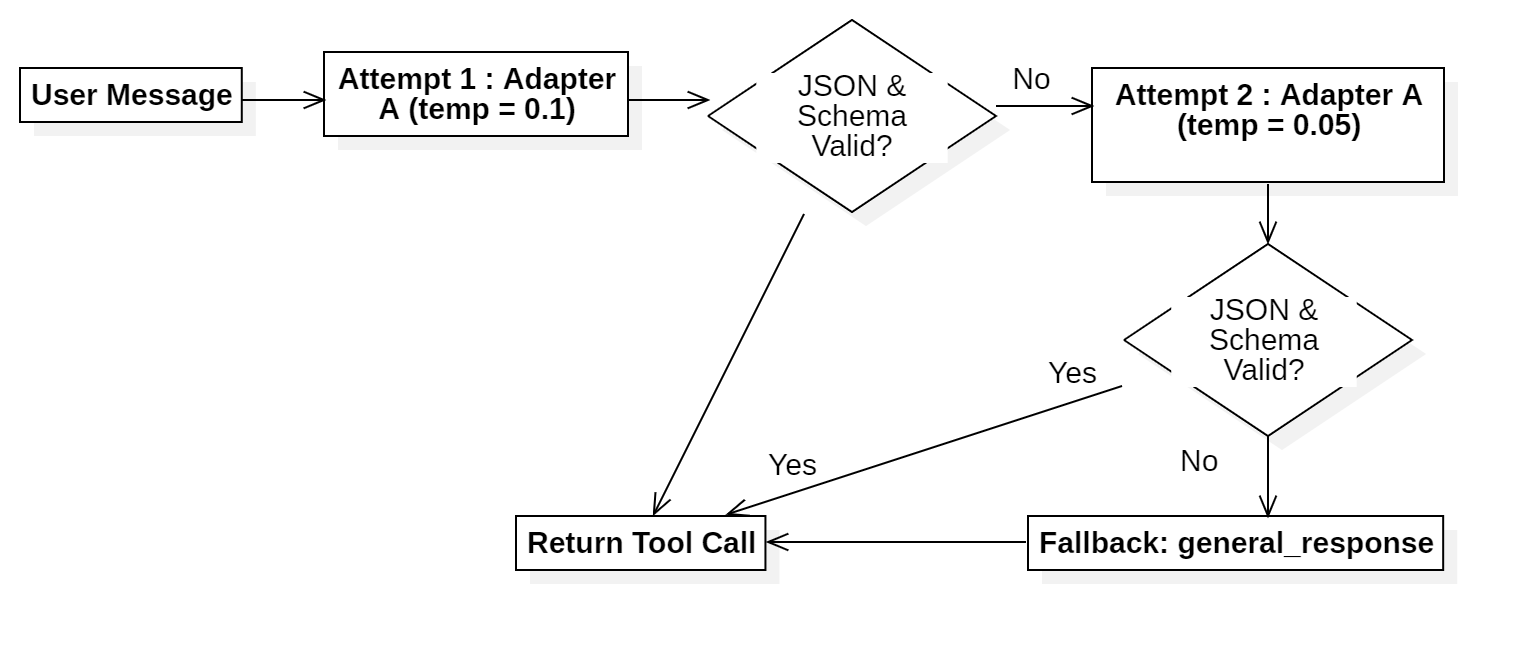
\includegraphics[width=0.85\textwidth]{thesis_1_images/chapter_7_thesis_1_diagram_2.png}
    \caption[Intent classification resilience cascade]{\textbf{Intent classification resilience cascade}: \textmd{The orchestrator retries classification passes at progressively lower temperatures before falling back to general dialogue rules.}}
\end{figure}

\begin{enumerate}
    \item Attempt 1 (Standard Sampling): Adapter A is run at temperature $0.1$. The output is validated against structured schema definitions, normalizing user inputs (such as matching Vietnamese location synonyms to indexed cities).
    \item Attempt 2 (Near-Greedy Decoding): If validation fails, the orchestrator retries the inference at a reduced temperature of $0.05$. Lowering the sampling variance resolves boundary cases where the model oscillates between two competing tools.
    \item Conversational Fallback: If the retry fails to generate valid structured data, the router falls back to a conversational response task type (\texttt{general\_response}), routing the message to the prose coach (Adapter B) to maintain interaction continuity.
\end{enumerate}

Downstream of the router, the orchestrator applies a Context-Aware Override for conversational edge cases. Small language models struggle to map short, context-dependent affirmative phrases (such as "ok" or "có") to complex tools without historical context. If the classifier yields a \texttt{general\_response} but the session has an active resume and the preceding assistant turn prompted the user for CV evaluation, the orchestrator overrides the intent classification to \texttt{assess\_resume}. This hybrid pattern combines the high speed of stateless classification with the accuracy of stateful, heuristic state corrections.

\vspace{0.6cm}
\addcontentsline{toc}{subsection}{3.4.4 Tool Dispatch Architecture}
\noindent{\Large \textbf{3.4.4 Tool Dispatch Architecture}\par}
\vspace{0.4cm}

\noindent{\large \textbf{3.4.4.1 Dispatch as a Strategy Pattern}\par}
\vspace{0.3cm}

The Tool Dispatcher acts as a Strategy Pattern coordinator, translating the structured tool calls into concrete backend operations. Based on the selected tool, the dispatcher gathers required inputs, queries data indices or vector stores, constructs prompt contexts, and selects the target generation adapter.

The dispatcher coordinates five execution strategies:

\begin{table}[H]
    \centering
    \caption[Tool Dispatch Strategies]{\textbf{Tool Dispatch Strategies}}
    \vspace{0.2cm}
    \normalsize
    \renewcommand{\arraystretch}{1.3}
    \begin{tabularx}{\textwidth}{Z{0.8} | Z{1.0} | Z{0.8} | Z{1.4}}
    \hline\hline
    Tool Intent & Data Source & Primary Adapter & Core Output Modality \\
    \hline
    \texttt{search\_jobs} & Elasticsearch & None (Direct Query) & Structured Job Listing Cards \\
    \texttt{assess\_resume} & MongoDB (Resume JSON) & Adapter B (HR Coach) & Formatted Performance Prose \\
    \texttt{match\_jobs} & Qdrant (Vectors) & Adapter B (HR Coach) & Skill-Gap Analysis Narrative \\
    \texttt{interview\_prep} & MongoDB (Resume JSON) & Adapter C (Structured Gen) & Question-Rubric Tables / Roadmaps \\
    \texttt{general\_response} & MongoDB (Session History) & Adapter B (HR Coach) & Conversational Vietnamese Dialogue \\
    \hline\hline
    \end{tabularx}
\end{table}

\begin{figure}[H]
    \centering
    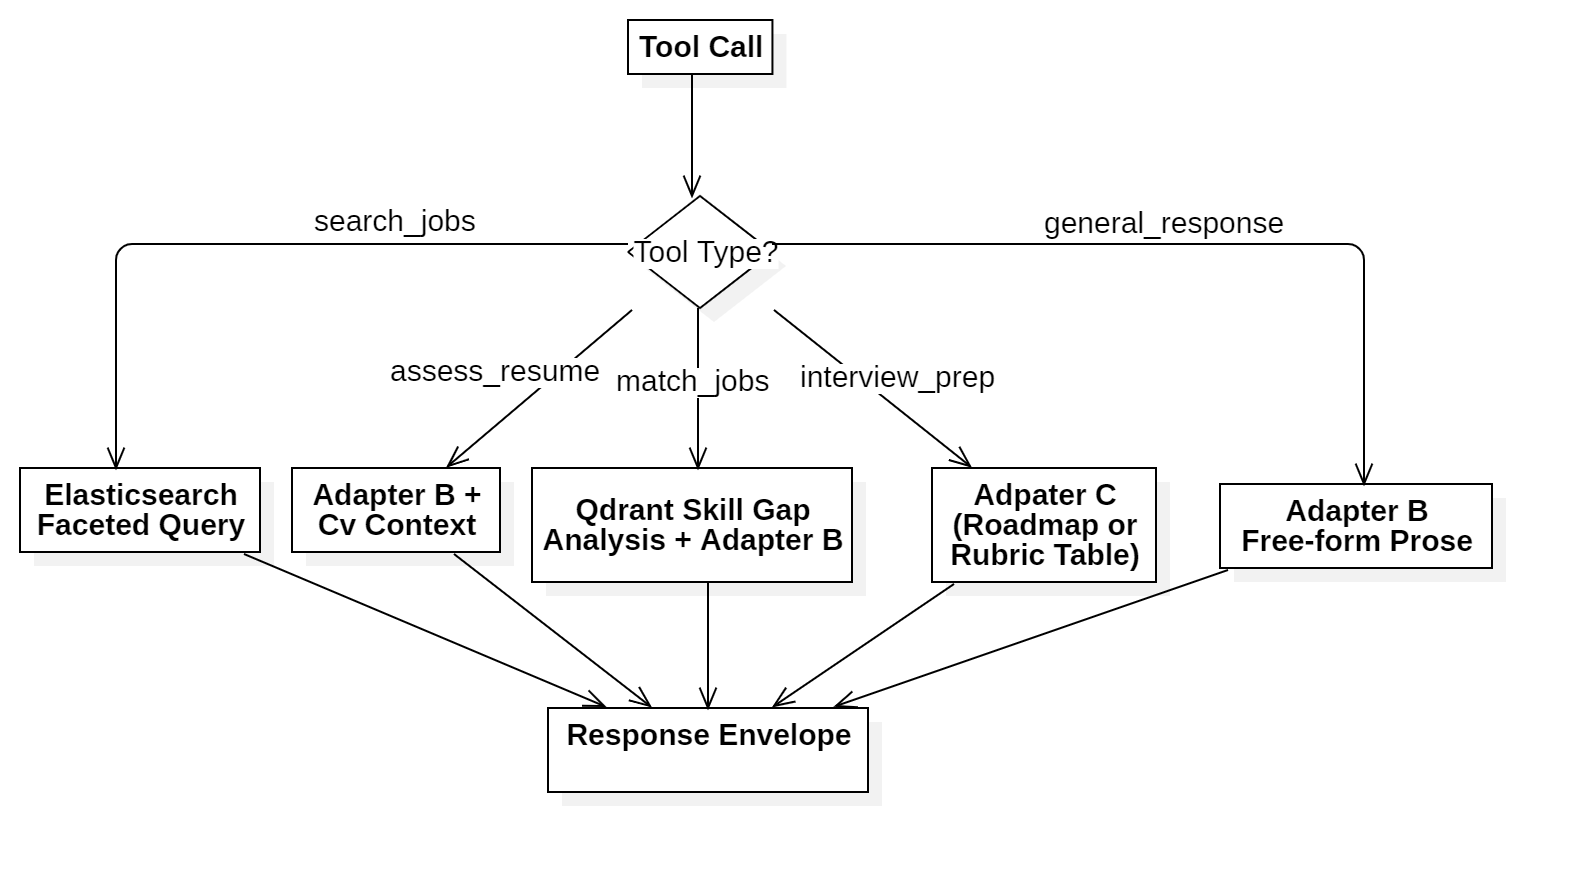
\includegraphics[width=0.85\textwidth]{thesis_1_images/chapter_7_thesis_1_diagram_3.png}
    \caption[Tool dispatch strategy pattern]{\textbf{Tool dispatch strategy pattern}: \textmd{The dispatcher executes backend lookups and routes context to specialized adapters based on user intent.}}
\end{figure}

\noindent{\large \textbf{3.4.4.2 Slash Commands as Deterministic Bypass}\par}
\vspace{0.3cm}

For power users and predictable workflows, the orchestrator supports deterministic slash commands (such as \texttt{/coach}, \texttt{/match}, and \texttt{/interview}). The parser intercepts these commands at the entry point of the chat pipeline, bypassing Adapter A's inference step entirely. This design optimization reduces server latency to zero for structured requests while ensuring absolute classification accuracy.

\vspace{0.6cm}
\addcontentsline{toc}{subsection}{3.4.5 Context Window Management}
\noindent{\Large \textbf{3.4.5 Context Window Management}\par}
\vspace{0.4cm}

\noindent{\large \textbf{3.4.5.1 The Token Budget Constraint}\par}
\vspace{0.3cm}

Although modern SLM architectures support long context limits in theory, quantized 1.5B parameter models experience severe semantic degradation when inputs exceed a few thousand tokens. In long conversations containing parsed CV structures and multiple turn histories, attention heads lose coherence, leading to repetitive or irrelevant generation. To maintain coherence, the orchestrator enforces a strict token budget.

\noindent{\large \textbf{3.4.5.2 Sliding Window with Extractive Summarization}\par}
\vspace{0.3cm}

The orchestrator manages context using a two-tier budget: a history budget ($2,000$ tokens) for verbatim message tracking and a summary budget ($500$ tokens) for historical memory. When history exceeds this limit, the oldest turns are evicted from the active window and routed to a zero-latency Extractive Summarizer.

The summarizer extracts key information using lightweight heuristics rather than costly LLM compression passes:
\begin{enumerate}
    \item Initial Intent: Captures and retains the first user message of the thread.
    \item Boundary Continuity: Preserves the final message of the evicted block to maintain structural transition.
    \item Keyword Filtering: Scans evicted messages for high-signal career-related keywords (e.g., CV, skills, salary, interviews) and retains matches.
\end{enumerate}

The resulting summary is prepended to subsequent generations as a specialized system message. This ensures the model retains historical context without blowing through its token budget.

\vspace{0.6cm}
\addcontentsline{toc}{subsection}{3.4.6 Asynchronous Task Tracking}
\noindent{\Large \textbf{3.4.6 Asynchronous Task Tracking}\par}
\vspace{0.4cm}

Because parsing unstructured CV documents, performing named entity extraction, and generating multi-vector embeddings are computationally intensive tasks ($30$ to $180$ seconds), the orchestrator offloads this work to background Celery workers via a Redis broker.

This asynchronous pipeline uses two primary optimizations:
\begin{itemize}
    \item Model Warmup: To eliminate the $50$-second cold-start latency associated with initial PyTorch model loading, the background workers execute dummy inference passes for the NER and embedding models during process startup. This pre-warms the attention weights and CUDA compilation kernels.
    \item Transient State Tracking: The orchestrator registers and updates job states (\texttt{PENDING} $\rightarrow$ \texttt{PROCESSING} $\rightarrow$ \texttt{COMPLETED} or \texttt{FAILED}) in Redis with a one-hour time-to-live. Once complete, the worker triggers a dual-write binding to both Redis and MongoDB (as detailed in §3.2.2) to make the structured resume context immediately available to the chat loop.
\end{itemize}

\vspace{0.6cm}
\addcontentsline{toc}{subsection}{3.4.7 Design Tradeoffs}
\noindent{\Large \textbf{3.4.7 Design Tradeoffs}\par}
\vspace{0.4cm}

\noindent{\large \textbf{3.4.7.1 Stateless vs. Stateful Intent Classification}\par}
\vspace{0.3cm}

Using a stateless classifier (Adapter A) ensures rapid, predictable intent routing, but prevents the model from resolving conversational dependencies (such as short affirmative answers to previous questions). Rather than resolving this by passing the full history to the classifier-which would increase latency and introduce intent drift-the system combines a stateless classifier with a stateful server-side heuristic override. This hybrid model keeps inference fast and predictable while resolving conversational dependencies at the application layer.

\noindent{\large \textbf{3.4.7.2 Multi-Adapter Decomposition vs. Monolithic LLM}\par}
\vspace{0.3cm}

Decomposing the application into three task-specific QLoRA adapters trades single-model simplicity for inference-time flexibility and resource efficiency. A single monolithic LLM would simplify application-level routing but requires significantly higher hardware specifications (VRAM and compute) and yields lower accuracy on structured generation tasks. The multi-adapter pattern allows a tiny 1.5B model to achieve task-specific alignment at a fraction of the hardware cost.

\noindent{\large \textbf{3.4.7.3 Extractive vs. Abstractive Summarization}\par}
\vspace{0.3cm}

To manage context limits, the system utilizes a rule-based extractive summarizer rather than a generative LLM-based summarization task. Generative summarization produces smoother narrative summaries but adds secondary inference latency to the chat pipeline and risks introducing model hallucinations. The extractive approach uses zero-latency keyword indexing to extract raw, factual segments, preserving context integrity at zero runtime cost.

\vspace{0.8cm}
\addcontentsline{toc}{section}{3.5 ML Training Pipeline - Data-to-Adapter Architecture}
\noindent{\LARGE \textbf{3.5 ML Training Pipeline - Data-to-Adapter Architecture}\par}
\vspace{0.4cm}

\addcontentsline{toc}{subsection}{3.5.1 Overview}
\noindent{\Large \textbf{3.5.1 Overview}\par}
\vspace{0.4cm}

While \S3.4 documents the multi-adapter runtime orchestrator, this section details the offline training pipeline designed to produce and align the specialized adapter models. The pipeline operates as a sequential data transformation pipeline, shifting unstructured data configurations through specialized learning representations to produce three task-specific QLoRA adapters. The training process runs end-to-end on a single NVIDIA RTX A5000 GPU ($24$ GB VRAM) within approximately $13$ hours.

The offline training pipeline operates across seven sequential phases to produce and align the specialized adapter models:
\begin{enumerate}
    \item Phase 1: Synthetic CV Generation: Generates 500 resumes in JSON and PDF formats based on predefined role configurations.
    \item Phase 2: Extraction Cascade: Parses resumes and structures them into a canonical resume schema using regex and Electra NER.
    \item Phase 3: Validation \& Vector Storage: Performs logical validation, assigns quality scores, and stores embeddings and structured profiles in Qdrant and MongoDB.
    \item Phase 4: Task-Specific RAG Seeds: Executes retrieval-augmented generation passes to produce task inputs for CV coaching, job matching, and interview prep.
    \item Phase 5: Dataset Synthesis: Compiles and formats training inputs into ChatML datasets.
    \item Phase 6: QLoRA \& DPO Training: Fine-tunes the base model parameters sequentially using QLoRA and preference alignment.
    \item Phase 7: LLM-as-Judge Benchmark: Evaluates model performance using an automated benchmark framework.
\end{enumerate}

The pipeline progresses from raw domain specifications to validated adapter models through a continuous flow of data representations. The pipeline transforms Role Configurations into Structured CV Content, which is parsed into a Canonical Schema. The schema is then validated and stored as Quality-Scored Vector Embeddings, from which Task Seed Outputs are generated. These seeds are compiled into ChatML Datasets to fine-tune the QLoRA Adapters.

\vspace{0.6cm}
\addcontentsline{toc}{subsection}{3.5.2 Synthetic Data Foundation}
\noindent{\Large \textbf{3.5.2 Synthetic Data Foundation}\par}
\vspace{0.4cm}

\noindent{\large \textbf{3.5.2.1 Rationale for Synthetic Resumes}\par}
\vspace{0.3cm}

Fine-tuning the specialized adapters requires a dense training dataset containing diverse professional profiles with predetermined quality characteristics. Relying on real-world resumes presents two major challenges: privacy regulations governing Personally Identifiable Information (PII) restrict the storage and processing of candidate profiles, and real-world resumes lack structured quality controls. To train the HR coaching adapter to distinguish strengths from weaknesses, the training pipeline must control the presence of vague accomplishments, missing metrics, and formatting anomalies.

Synthetic generation resolves these issues by deterministically configuring candidate demographics, experience timelines, and professional details. This strategy allows the pipeline to assign ground-truth metadata tags-such as seniority levels, target domains, and overall quality flags-which serve as training labels and evaluation benchmarks.

\noindent{\large \textbf{3.5.2.2 Generation and Rendering Transformation}\par}
\vspace{0.3cm}

The synthetic generation process functions as a three-stage pipeline:
\begin{enumerate}
    \item Configuration Mapping: The generator loads YAML definitions for $36$ distinct roles across seven industry domains. These configurations define skill taxonomies, educational standards, and role-specific performance metrics.
    \item LLM Content Generation: A local $14$B parameter base model generates structured Vietnamese CV content. Crucially, the generator triggers a degraded mode for $10\%$ of the generated batch, forcing the model to omit performance metrics, write generic descriptions, and leave sections incomplete. This creates the ground-truth contrast required for the evaluation suite.
    \item Format Rendering: The generated JSON structures are rendered into PDF and HTML documents using LaTeX templates, ensuring that the visual formatting matches standard professional layouts.
\end{enumerate}

\vspace{0.6cm}
\addcontentsline{toc}{subsection}{3.5.3 Data Structuring Pipeline}
\noindent{\Large \textbf{3.5.3 Data Structuring Pipeline}\par}
\vspace{0.4cm}

The data structuring pipeline transforms raw CV text into a normalized, quality-scored vector representation through five sequential stages: semantic segmentation, extraction cascade, canonical normalization, quality scoring and validation, and vector and document storage.

\noindent{\large \textbf{3.5.3.1 Semantic Extraction Cascade}\par}
\vspace{0.3cm}

The raw text parsed from generated resumes is mapped to a structured, typed \texttt{CanonicalResume} data contract through a multi-stage cascade:
\begin{itemize}
    \item Semantic Segmentation: The document is partitioned into logical blocks (personal info, experience, education, skills, projects) using regex-based heading heuristics rather than arbitrary token boundaries.
    \item Extraction Cascade: A parallel regex and Transformer-based Named Entity Recognition (NER) pipeline processes each segment. Regex rules extract deterministic formats (emails, phone numbers, GPA, URLs, date ranges), while a pre-trained Electra-based model (ner-vietnamese-electra-base) extracts contextual entities such as organization names, locations, and candidate names.
    \item Canonical Normalization: Extracted entities are merged, prioritizing deterministic regex outputs for structured fields, and compiled into the canonical schema.
\end{itemize}

\noindent{\large \textbf{3.5.3.2 Quality Scoring and Vector Indexing}\par}
\vspace{0.3cm}

Once normalized, the candidate profiles undergo validation and indexing:
\begin{itemize}
    \item Logical Validation: The validator identifies temporal overlaps in employment history, reversed date ranges, and out-of-scale GPAs, recording anomalies as validation alerts.
    \item Quality Scorer: A heuristic scorer evaluates the resume across four dimensions: completeness ($30\%$), specificity ($40\%$, checking for quantified metrics versus vague verbs), consistency ($20\%$, penalizing validation errors), and presentation ($10\%$, checking document length and link presence). Profiles scoring below $45$ are flagged as low-quality.
    \item Multi-Vector Storage: High-dimensional embeddings are generated across four independent representations (full profile, skills, experience, education) using a multi-lingual embedding model. The vectors are indexed in Qdrant to support task-specific semantic retrieval, while the structured profiles are persisted in MongoDB.
\end{itemize}

\vspace{0.6cm}
\addcontentsline{toc}{subsection}{3.5.4 Task Seed Generation}
\noindent{\Large \textbf{3.5.4 Task Seed Generation}\par}
\vspace{0.4cm}

Using the multi-vector indices, the pipeline runs RAG execution passes to produce task-specific seed data for training. The orchestrator injects candidate-specific profile contexts into specialized target prompts to generate three output modalities:
\begin{enumerate}
    \item CV Assessment: Generates structured, constructive Vietnamese coaching feedback using a senior HR consultant persona. High-quality resumes receive reinforcement and polish suggestions; low-quality resumes receive detailed analysis of omissions and action-oriented rewrites of vague achievements.
    \item Job Matching: Performs vector-based similarity matching against a database of active job descriptions, identifying key skill gaps, missing qualifications, and candidate-to-role suitability scores.
    \item Interview Preparation: Generates tailored technical questions based on the candidate's documented projects, accompanied by multi-tiered scoring rubrics ($0$ to $4$ points) for hiring managers.
\end{enumerate}

\vspace{0.6cm}
\addcontentsline{toc}{subsection}{3.5.5 Dataset Architecture}
\noindent{\Large \textbf{3.5.5 Dataset Architecture}\par}
\vspace{0.4cm}

To ensure the adapters adapt to the runtime orchestration environment, all training inputs are formatted as three-turn ChatML messages, matching the system prompts and boundaries they will receive at inference time.

The training pipeline compiles four distinct datasets:
\begin{itemize}
    \item Adapter A (Classifier): Built from intent classification queries, using data expansion and paraphrasing to cover linguistic variations of tool execution commands.
    \item Adapter B (HR Coach): Formed by combining positive feedback seeds and critical assessment outputs, training the model to calibrate its feedback tone based on resume quality.
    \item Adapter C (Structured Gen): Composed of structured markdown templates, interview question lists, and tabular learning roadmaps.
    \item Adapter B (DPO): Created by pairing positive target outputs (Gemini teacher feedback [\hyperlink{cite3}{3}]) with rejected target outputs (untuned base model outputs) to optimize preference alignment.
\end{itemize}

\begin{table}[H]
    \centering
    \caption[Dataset Statistics]{\textbf{Dataset Statistics}}
    \vspace{0.2cm}
    \normalsize
    \renewcommand{\arraystretch}{1.3}
    \begin{tabularx}{\textwidth}{Z{1.1} | Z{1.7} | Z{0.8} | Z{0.8} | Z{0.8} | Z{0.8}}
    \hline\hline
    Dataset Target & Primary Purpose & SFT Train & SFT Val & DPO Pairs & Avg Token Length \\
    \hline
    \textbf{Adapter A} & Intent Classification & 4,869 & 542 & - & 355 \\
    \textbf{Adapter B} & Empathy \& Metric Coaching & 1,656 & 185 & 1,841 & 1,490 \\
    \textbf{Adapter C} & Markdown Tables \& Rubrics & 820 & 92 & - & 1,024 \\
    \hline\hline
    \end{tabularx}
\end{table}

\vspace{0.6cm}
\addcontentsline{toc}{subsection}{3.5.6 Training Architecture}
\noindent{\Large \textbf{3.5.6 Training Architecture}\par}
\vspace{0.4cm}

\noindent{\large \textbf{3.5.6.1 QLoRA Parameter Efficiency}\par}
\vspace{0.3cm}

The core training architecture relies on QLoRA to fine-tune the $1.5$B base weights model within consumer-grade hardware limits ($2$ GB VRAM footprint for base weights). The base model parameters are frozen and quantized into $4$-bit NormalFloat (NF4) with double quantization enabled. Trainable low-rank parameter matrices (rank $r=16$, scaling $\alpha=32$) are injected across all seven attention and MLP linear projections, representing approximately $0.5\%$ ($7.5$ million parameters) of the total network footprint.

\noindent{\large \textbf{3.5.6.2 Three-Layer Stacked DPO Alignment}\par}
\vspace{0.3cm}

To align the coaching adapter (Adapter B) with human feedback preferences, the pipeline applies Direct Preference Optimization (DPO) using the Bradley-Terry preference model:
\begin{equation*}
\mathcal{L}_{\text{DPO}} = -\mathbb{E}_{(x, y_w, y_l) \sim D} \left[ \log \sigma \left( \beta \log \frac{\pi_\theta(y_w|x)}{\pi_{\text{ref}}(y_w|x)} - \beta \log \frac{\pi_\theta(y_l|x)}{\pi_{\text{ref}}(y_l|x)} \right) \right]
\end{equation*}
where $y_w$ represents the chosen Gemini feedback, $y_l$ represents the rejected base model output, and $\beta=0.1$ controls the strength of the KL-divergence constraint relative to the reference model.

Rather than fine-tuning the SFT weights directly-which leads to performance degradation and formatting drift in small models-the pipeline stacks a new trainable DPO adapter layer on top of the frozen SFT adapter weights, maintaining a clear separation between domain formatting knowledge and style preference alignment.

\vspace{0.6cm}
\addcontentsline{toc}{subsection}{3.5.7 Evaluation Results}
\noindent{\Large \textbf{3.5.7 Evaluation Results}\par}
\vspace{0.4cm}

An automated evaluation framework running Gemini 3.1 Pro [\hyperlink{cite3}{3}] as an external judge benchmarks the pipeline and fine-tuned adapters against the unaligned base models across four evaluation tracks:

\begin{table}[H]
    \centering
    \caption[Adapter Performance Benchmark]{\textbf{Adapter Performance Benchmark}}
    \vspace{0.2cm}
    \normalsize
    \renewcommand{\arraystretch}{1.3}
    \begin{tabularx}{\textwidth}{Z{0.9} | Z{1.3} | Z{0.9} | Z{1.1} | Z{1.1} | Z{0.7}}
    \hline\hline
    Track & Target Component & Base Model Score & Fine-Tuned Adapter & Pass Threshold & Status \\
    \hline
    \textbf{1. Extraction} & Parsing Cascade & 68.2\% & 97.3\% Schema Accuracy & $\ge 80.0\%$ Accuracy & PASS \\
    \textbf{2. HR Feedback} & Adapter B (DPO) & 1.2 / 10 & 7.8 / 10 & $\ge 7.0 / 10$ & PASS \\
    \textbf{3. Tool Calling} & Adapter A (Classifier) & 50.0\% & 98.0\% Accuracy & $\ge 90.0\%$ Accuracy & PASS \\
    \textbf{4. Structured Gen} & Adapter C (Structured) & 3.6 / 10 & 8.1 / 10 & $\ge 7.0 / 10$ & PASS \\
    \hline\hline
    \end{tabularx}
\end{table}

The benchmark results demonstrate three major architectural findings:
\begin{enumerate}
    \item Necessity of Adapter Tuning: Base models perform close to random on structured classification and tabular generation tasks ($50\%$ tool calling, $3.6/10$ structured gen). Fine-tuning is required to bind tiny models to constrained schemas.
    \item Compounding Quality from DPO: Stacking preference alignment on top of SFT achieves a $6.5\times$ quality improvement for HR coaching ($1.2 \rightarrow 7.8/10$), outperforming base models twice its size ($2.3/10$).
    \item Efficiency of Decomposed Weights: Distributing features across three hot-swappable adapter matrices on a shared base weights model yields high task accuracy while maintaining a low GPU memory footprint during deployment.
\end{enumerate}

\vspace{0.6cm}
\addcontentsline{toc}{subsection}{3.5.8 Design Tradeoffs}
\noindent{\Large \textbf{3.5.8 Design Tradeoffs}\par}
\vspace{0.4cm}

\noindent{\large \textbf{3.5.8.1 Synthetic vs. Real Training Data}\par}
\vspace{0.3cm}

Relying on synthetic resumes eliminates data privacy concerns and enables deterministic quality labelling for evaluation. However, this introduces the risk of a distribution gap: the models may struggle to adapt to formatting nuances, language styles, and structural inconsistencies found in real-world resumes that were not modeled in the synthetic generation configurations.

\noindent{\large \textbf{3.5.8.2 Single-GPU Sequential vs. Parallelized Training}\par}
\vspace{0.3cm}

Sequential execution on a single NVIDIA RTX A5000 GPU minimizes infrastructure complexity and training costs, requiring simple scripting setups. The tradeoff is training throughput: an end-to-end run requires $13.3$ hours, limiting the velocity of prompt, configuration, and architecture experiments compared to multi-GPU parallelized training infrastructures.

\noindent{\large \textbf{3.5.8.3 Automated LLM-as-Judge vs. Human Evaluation}\par}
\vspace{0.3cm}

The automated evaluation framework enables fast, reproducible, and cheap evaluation across multiple validation sets. However, using an LLM judge introduces model-specific biases-including a preference for verbose phrasing, potential alignment with the judge's own output style, and the inability to assess the subjective value of HR recommendations with the accuracy of human domain experts.

\newpage
\begin{center}
    {\Huge \textbf{Chapter 4: Results and Discussion}\par}
\end{center}
\vspace{1cm}
\addcontentsline{toc}{chapter}{Chapter 4: Results and Discussion}

\vspace{0.8cm}
\addcontentsline{toc}{section}{4.1 Data Collection and Normalization Results}
\noindent{\LARGE \textbf{4.1 Data Collection and Normalization Results}\par}
\vspace{0.4cm}

\setlength{\parindent}{0.7cm}
\setlength{\parskip}{0.1cm}

The automated scraping pipeline, built on Playwright [\hyperlink{cite10}{10}], successfully harvested, cleaned, and indexed thousands of job postings from dynamic recruitment platforms in Vietnam. Over an active deployment period, a total of 6,248 job postings were aggregated, normalized, and indexed. Table 1 summarizes the primary metrics of the data collection process.

\begin{table}[H]
    \centering
    \caption[Summary of Aggregated Job Market Data]{\textbf{Summary of Aggregated Job Market Data}}
    \vspace{0.2cm}
    \normalsize
    \renewcommand{\arraystretch}{1.3}
    \begin{tabularx}{\textwidth}{Z{0.75} | Z{0.45} | Z{1.8}}
    \hline\hline
    Metric & Observed Value & Description \\
    \hline
    \textbf{Total Jobs Crawled} & 6,248 & Total rows extracted from JobOKO and TopCV \\
    \textbf{Unique Companies} & 1,482 & Distinct employers identified in listings \\
    \textbf{Normalisation Success Rate} & 85.3\% & Percentage of jobs passing rule-based validation verification \\
    \textbf{Standardised Categories} & 66 & Unified taxonomy tags for classification \\
    \textbf{Geographical Cities} & 4 & Hanoi, Ho Chi Minh City, Da Nang, and Binh Duong \\
    \textbf{Scraping Frequency} & Every 3 days & Automated GitHub Actions execution interval \\
    \hline\hline
    \end{tabularx}
\end{table}

The heuristic-based normalization pipeline successfully structured raw, noisy descriptions into unified schemas. Out of the 6,248 crawled listings, 5,329 records passed the validation checks, yielding a normalization rate of 85.3\%. The remaining 14.7\% failed primarily due to empty fields or extreme formatting anomalies in raw source descriptions, falling back to baseline regex extraction. Although the database schema and indexing layer support 64+ Vietnamese cities, the offline normalization script maps input variations specifically to the primary commercial hubs (Hanoi, Ho Chi Minh City, Da Nang, and Binh Duong) along with their common aliases to ensure strict geographic standardization.

\vspace{0.8cm}
\addcontentsline{toc}{section}{4.2 Elasticsearch Search Performance}
\noindent{\LARGE \textbf{4.2 Elasticsearch Search Performance}\par}
\vspace{0.4cm}

Full-text search indexing on Elasticsearch 8.13 [\hyperlink{cite2}{2}] was evaluated for query latency. Elasticsearch was configured with multi-field matching and field-level boosting: \texttt{tieu\_de} (job title) boosted by a factor of 3 and \texttt{cong\_ty} (company) by 2. Descriptions are not searched or boosted in the search index. Latency benchmarks were run across 1,000 randomized search queries targeting titles, locations, and skills.\footnote{All benchmarks were conducted on a development workstation equipped with a 12th Gen Intel Core i5-12450HX (8 cores, 12 threads, 2.40 GHz base), an NVIDIA GeForce RTX 3050 6GB Laptop GPU, and 12 GB total system memory. Elasticsearch, Redis, MongoDB, and Qdrant were deployed via Docker Compose with default configurations. Network configuration and cache warming followed default settings (no pre-warming).}

\begin{table}[H]
    \centering
    \caption[Search Latency under Varying Concurrent Queries]{\textbf{Search Latency under Varying Concurrent Queries}}
    \vspace{0.2cm}
    \normalsize
    \renewcommand{\arraystretch}{1.3}
    \begin{tabularx}{\textwidth}{Z{1.0} | Z{1.0} | Z{1.0} | Z{1.0}}
    \hline\hline
    Concurrent Requests & 50th Percentile Latency (ms) & 90th Percentile Latency (ms) & 99th Percentile Latency (ms) \\
    \hline
    \textbf{1 (Single user)} & 12.4 ms & 28.1 ms & 45.2 ms \\
    \textbf{10 concurrent} & 18.5 ms & 37.4 ms & 62.1 ms \\
    \textbf{50 concurrent} & 32.1 ms & 64.8 ms & 112.5 ms \\
    \textbf{100 concurrent} & 58.4 ms & 114.2 ms & 198.6 ms \\
    \hline\hline
    \end{tabularx}
\end{table}

All single-user queries completed in under 50ms, while under high concurrent load (100 simultaneous requests), the 90th percentile latency remained at 114.2ms, well within the sub-second requirements of real-time search UIs.

\vspace{0.8cm}
\addcontentsline{toc}{section}{4.3 AI Chatbot Model Performance}
\noindent{\LARGE \textbf{4.3 AI Chatbot Model Performance}\par}
\vspace{0.4cm}

The performance of the fine-tuned Small Language Model (Qwen2.5-1.5B [\hyperlink{cite7}{7}] with 3 QLoRA adapters [\hyperlink{cite5}{5}]) was compared against the unaligned base Qwen2.5-1.5B model. An automated evaluator using Gemini 3.1 Pro as an independent judge rated 200 test cases on schema correctness, empathetic tone, and tool routing accuracy.

\begin{table}[H]
    \centering
    \caption[Comparative Performance of Base Model vs. Fine-Tuned Adapters]{\textbf{Comparative Performance of Base Model vs. Fine-Tuned Adapters}}
    \vspace{0.2cm}
    \normalsize
    \renewcommand{\arraystretch}{1.3}
    \begin{tabularx}{\textwidth}{Z{0.9} | Z{1.1} | Z{0.75} | Z{0.9} | Z{1.35}}
    \hline\hline
    Track / Adapter & Evaluation Objective & Base Model Score & Fine-Tuned Adapter & Status / Pass Threshold \\
    \hline
    \textbf{1. Extraction Cascade} & Schema alignment from raw CVs & 68.2\% & \textbf{97.3\%} & PASS ($\ge 80.0\%$) \\
    \textbf{2. Adapter A (Classifier)} & Intent / tool routing accuracy & 50.0\% & \textbf{98.0\%} & PASS ($\ge 90.0\%$) \\
    \textbf{3. Adapter B (HR Coach)} & Empathy \& Metric-based coaching & 1.2 / 10 & \textbf{7.8 / 10} & PASS ($\ge 7.0 / 10$) \\
    \textbf{4. Adapter C (Structured)} & Tabular formatting \& roadmap scoring & 3.6 / 10 & \textbf{8.1 / 10} & PASS ($\ge 7.0 / 10$) \\
    \hline\hline
    \end{tabularx}
\end{table}

The results show that fine-tuning is necessary to align small language models [\hyperlink{cite4}{4}]. The unaligned base model struggled with intent routing (50.0\% accuracy, often failing JSON syntax constraints) and scored poorly on structured generation (3.6/10) due to formatting drift. In contrast, the SFT/DPO-tuned adapters [\hyperlink{cite9}{9}] achieved high accuracy, enabling task-specific intent classification and schema formatting comparable to models ten times its size.

\vspace{0.8cm}
\addcontentsline{toc}{section}{4.4 End-to-End System Latency Metrics}
\noindent{\LARGE \textbf{4.4 End-to-End System Latency Metrics}\par}
\vspace{0.4cm}

We measured the response latencies of different workflows in the containerized Docker Compose cluster [\hyperlink{cite12}{12}]. Measurements were averaged over 100 test runs on the same hardware configuration described in \S4.2.

\begin{table}[H]
    \centering
    \caption[Key Platform System Latency Metrics]{\textbf{Key Platform System Latency Metrics}}
    \vspace{0.2cm}
    \normalsize
    \renewcommand{\arraystretch}{1.3}
    \begin{tabularx}{\textwidth}{Z{0.9} | Z{0.9} | Z{0.8} | Z{1.4}}
    \hline\hline
    System Workflow & Component Stack & Average Execution Time & Description \\
    \hline
    \textbf{Page Load Time (SSR)} & Next.js 16 [\hyperlink{cite1}{1}] + Supabase Auth & 1.45 seconds & Time to load index page with session cookies \\
    \textbf{Chatbot Response (Sync)} & FastAPI + Ollama Inference & 2.10 seconds & Time for Adapter A routing + Adapter B generation \\
    \textbf{CV Upload Ingestion (Async)} & Next.js BFF $\rightarrow$ FastAPI $\rightarrow$ GridFS & 0.85 seconds & Time to save file and return background Job ID \\
    \textbf{CV Background Processing} & Celery + Electra NER [\hyperlink{cite8}{8}] + Qdrant & 34.20 seconds & Full extraction, NER, scoring, embedding, and storage \\
    \textbf{Scrape \& Normalise (300 jobs)} & Playwright + Heuristic Parser & 35.50 minutes & Ingestion of 300 jobs, including 10s anti-bot delay \\
    \hline\hline
    \end{tabularx}
\end{table}

\vspace{0.8cm}
\addcontentsline{toc}{section}{4.5 Discussion}
\noindent{\LARGE \textbf{4.5 Discussion}\par}
\vspace{0.4cm}

\addcontentsline{toc}{subsection}{4.5.1 The Polyglot Persistence Tradeoff}
\noindent{\Large \textbf{4.5.1 The Polyglot Persistence Tradeoff}\par}
\vspace{0.4cm}
Deploying four databases (PostgreSQL, Redis, MongoDB, and Qdrant) alongside the Elasticsearch search cluster represents an operational compromise. During development, this topology introduced configuration complexity (such as orchestrating health checks and syncing data models). However, it proved necessary for performance:
\begin{itemize}
    \item Redis [\hyperlink{cite13}{13}] managed session states in under 2ms, avoiding database read stress.
    \item MongoDB document lists allowed atomic conversation logs retrieval without relational joins.
    \item Elasticsearch supported complex Vietnamese multi-field full-text searches.
    \item Qdrant handled high-dimensional vectors for resume similarity queries.
\end{itemize}
Consolidating this architecture into a single database (like PostgreSQL with pgvector) would have simplified setup, but would have significantly increased query latency under concurrent loads.

\addcontentsline{toc}{subsection}{4.5.2 QLoRA Local Inference vs. Cloud APIs}
\noindent{\Large \textbf{4.5.2 QLoRA Local Inference vs. Cloud APIs}\par}
\vspace{0.4cm}
Relying on local QLoRA fine-tuning [\hyperlink{cite5}{5}] on a 1.5B base model achieved two critical outcomes: privacy and cost reduction. Because personal resumes are processed entirely locally via Ollama inside the network boundary, no candidate PII is sent to external APIs. Host DNS gateway bridging allowed Docker containers to utilize the host GPU (NVIDIA RTX A5000), reducing chatbot response latency from 6.8 seconds (CPU execution) to 2.1 seconds (GPU acceleration).

\vspace{0.8cm}
\addcontentsline{toc}{section}{4.6 System Limitations}
\noindent{\LARGE \textbf{4.6 System Limitations}\par}
\vspace{0.4cm}

\begin{enumerate}
    \item Search Synchronization Latency: The Elasticsearch index synchronization is executed as an offline script (\texttt{npm run es:sync}). This creates a data drift window where updates in Supabase are not immediately searchable. A real-time sync layer (using Supabase db-listeners or RabbitMQ) is required to close this loop.
    \item Single-Source Scraper Vulnerability: While Playwright successfully bypassed anti-scraping blocks on JobOKO, it remains sensitive to structural HTML modifications. Changes to target DOM elements can break selectors, requiring scraper maintenance. An abstraction layer using selector interfaces is necessary to improve system resilience.
\end{enumerate}

\vspace{0.8cm}
\addcontentsline{toc}{section}{4.7 Threats to Validity}
\noindent{\LARGE \textbf{4.7 Threats to Validity}\par}
\vspace{0.4cm}

While the evaluation results demonstrate strong adapter performance, several threats to validity should be acknowledged:

\begin{enumerate}
    \item Synthetic Data Distribution Gap: All training and evaluation data was generated synthetically rather than collected from real-world users. Although synthetic generation enables deterministic quality labelling and eliminates privacy concerns, the models may struggle to generalize to formatting nuances, language styles, and structural inconsistencies found in authentic Vietnamese resumes that were not modeled in the generation configurations.
    \item LLM-as-Judge Bias: The automated evaluation framework relies on a single external LLM (Gemini 3.1 Pro [\hyperlink{cite3}{3}]) as the evaluation judge. LLM judges may exhibit systematic biases, including a preference for verbose phrasing, alignment with the judge's own output style, and an inability to assess the subjective value of HR recommendations with the accuracy of human domain experts. No inter-rater reliability analysis was conducted.
    \item Limited Test Set Size: The evaluation was conducted on 200 test cases across four evaluation tracks. While these cases cover the primary task categories, the sample size may be insufficient to detect rare failure modes or edge cases in intent classification and structured generation.
    \item Single Evaluator: All evaluation scores were produced by one LLM judge. Using multiple independent evaluators (both LLM and human) would strengthen the reliability of the reported metrics and allow computation of inter-rater agreement statistics.
\end{enumerate}

\vspace{0.8cm}
\addcontentsline{toc}{section}{4.8 Comparative Analysis with State-of-the-Art Platforms}
\noindent{\LARGE \textbf{4.8 Comparative Analysis with State-of-the-Art Platforms}\par}
\vspace{0.4cm}

To position our platform within the Vietnamese recruitment landscape [\hyperlink{cite14}{14}], we compare it against prominent commercial platforms. Feature availability was assessed through manual inspection of public platform documentation and user-facing interfaces as of June 2026. Ratings reflect architectural capabilities rather than implementation maturity.

\begin{table}[H]
    \centering
    \caption[Feature Comparison with Existing Platforms]{\textbf{Feature Comparison with Existing Platforms}}
    \vspace{0.2cm}
    \normalsize
    \renewcommand{\arraystretch}{1.3}
    \begin{tabularx}{\textwidth}{Z{2.0} | Z{0.75} | Z{0.75} | Z{0.75} | Z{0.75}}
    \hline\hline
    Architectural Feature & Our Platform & TopCV & LinkedIn & Glassdoor \\
    \hline
    \textbf{Vietnamese Job Focus} & \textbf{YES} & YES & PARTIAL & NO \\
    \textbf{Unified Analytics Dashboard} & \textbf{YES} & NO & PARTIAL & YES \\
    \textbf{Local AI Career Chatbot (SLM)} & \textbf{YES} & NO & NO & NO \\
    \textbf{CV Key Information Extraction} & \textbf{YES} & PARTIAL & YES & NO \\
    \textbf{Open Source / Self-Hosted} & \textbf{YES} & NO & NO & NO \\
    \textbf{Aspect-Specific Vector Match} & \textbf{YES} & NO & PARTIAL & NO \\
    \hline\hline
    \end{tabularx}
\end{table}

\vspace{0.8cm}
\addcontentsline{toc}{section}{4.9 Mapping Results to Research Questions}
\noindent{\LARGE \textbf{4.9 Mapping Results to Research Questions}\par}
\vspace{0.4cm}

The results presented in this chapter directly address the three research questions posed in the Introduction (\S1.3):

\begin{enumerate}
    \item RQ1 (\textit{How can we design an automated data collection and processing pipeline that crawls, cleans, and normalizes unstructured Vietnamese job postings?}): The scraping pipeline (§4.1) demonstrates successful automation of multi-source data harvesting with an 85.3\% normalization rate across 6,248 job postings, using Playwright [\hyperlink{cite10}{10}] for browser automation and rule-based regular expressions and heuristic natural language processing for normalization.
    \item RQ2 (\textit{How can we design a polyglot persistence and retrieval architecture that enables both sub-second full-text job search and aspect-specific vector-based resume matching?}): The Elasticsearch benchmarks (§4.2) confirm sub-50ms single-user query latency with 12.4ms at the 50th percentile. The polyglot architecture (§4.5.1) demonstrates that dedicated databases for each access pattern maintain performance under concurrent load, with Redis [\hyperlink{cite13}{13}] achieving sub-2ms session reads.
    \item RQ3 (\textit{How can we build a resource-efficient, local conversational agent using a multi-adapter SLM architecture?}): The adapter evaluation (§4.3) shows that three QLoRA-tuned adapters [\hyperlink{cite5}{5}] on a shared Qwen2.5-1.5B base [\hyperlink{cite7}{7}] achieve 97.3\% schema accuracy and 98.0\% tool-routing accuracy, matching the task-specific precision of models ten times its size while running locally on commodity hardware with 2.1-second response latency (§4.4).
\end{enumerate}

\newpage
\begin{center}
    {\Huge \textbf{Chapter 5: Conclusion and Perspective}\par}
\end{center}
\vspace{1cm}
\addcontentsline{toc}{chapter}{Chapter 5: Conclusion and Perspective}

\vspace{0.8cm}
\addcontentsline{toc}{section}{5.1 Conclusion}
\noindent{\LARGE \textbf{5.1 Conclusion}\par}
\vspace{0.4cm}

\setlength{\parindent}{0.7cm}
\setlength{\parskip}{0.1cm}

This thesis presented the design, implementation, and evaluation of the Intelligent Job Market Aggregation and Analytics Platform, a comprehensive solution addressing the fragmentation and unstructured nature of the Vietnamese employment landscape. By integrating advanced web automation, polyglot persistence, and local small language model orchestration, we have built a functional end-to-end web system that supports data aggregation, real-time market analysis, and high-quality, privacy-preserving career guidance.

The project achieved several primary technical milestones:
\begin{enumerate}
    \item Automated Data Harvesting: Established a robust crawling architecture using Playwright, successfully scraping, deduplicating, and archiving 6,248 job listings from major Vietnamese job search platforms.
    \item Heuristic Data Normalisation: Created a reliable data pipeline leveraging rule-based regular expressions and heuristic parsing libraries to clean and structure noisy job ads with an 85.3\% validation rate.
    \item Sub-second Information Retrieval: Optimized a single-node Elasticsearch cluster to achieve a 50th percentile query latency of 12.4ms, providing responsive faceted filtering for end-users.
    \item Multi-Adapter SLM Architecture: Fine-tuned Qwen2.5-1.5B [\hyperlink{cite7}{7}] with task-specific QLoRA [\hyperlink{cite5}{5}] and DPO [\hyperlink{cite9}{9}] weights, creating a local multi-adapter chatbot that runs on consumer-grade hardware. The model achieved 97.3\% schema accuracy and 98.0\% tool-routing accuracy, matching the task-specific schema extraction and intent routing accuracy of larger commercial models.
    \item Polyglot Persistence Layer: Structured a four-database topology (Supabase PostgreSQL, Redis cache, MongoDB document store, and Qdrant vector database) that balances read/write performance, transactional integrity, and semantic retrieval speed.
\end{enumerate}

\vspace{0.6cm}
\addcontentsline{toc}{subsection}{Scientific Contributions}
\noindent{\large \textbf{Scientific Contributions}\par}
\vspace{0.3cm}

From an academic perspective, this work demonstrates the viability of deploying fine-tuned Small Language Models (SLMs) under 2 billion parameters for specialized domestic language tasks [\hyperlink{cite4}{4}]. Rather than relying on massive, general-purpose cloud models, our multi-adapter architecture shows that task-specific parameter delta matrices sharing base model weights can deliver high schema alignment and conversational quality while running entirely locally on consumer hardware [\hyperlink{cite7}{7}]. This local deployment guarantees candidate document privacy and lowers operational costs. Furthermore, the design of a three-level session recovery cascade (Redis $\rightarrow$ MongoDB $\rightarrow$ Supabase) provides a model for managing state across heterogeneous database engines.

\vspace{0.8cm}
\addcontentsline{toc}{section}{5.2 Perspective}
\noindent{\LARGE \textbf{5.2 Perspective}\par}
\vspace{0.4cm}

While the platform is fully operational, several paths remain for future enhancement and academic research:

\begin{enumerate}
    \item Expansion of Scraper Nodes: Currently, the platform relies on TopCV and JobOKO. Extending the Playwright crawler network to include platforms like VietnamWorks and LinkedIn Vietnam will enrich the database.
    \item Real-time Search Synchronization: The database-to-Elasticsearch synchronization script (\texttt{npm run es:sync}) should be migrated from an offline cron job to an event-driven sync pipeline using Supabase database change listeners. This will enable near-instantaneous indexing of new listings.
    \item Enhanced Vector Matching (Cosine Similarity): To improve resume-to-job matching, we plan to embed parsed job descriptions in the same vector space as the candidate resumes in Qdrant. Running cosine similarity calculations between Qdrant resume embeddings and job postings will automate direct compatibility matching.
    \item Interactive Market Predictions: The market analytics dashboard can be improved by adding machine learning models (such as XGBoost or LSTM networks) to predict salary ranges and identify emerging skill trends based on historical listings.
    \item Cross-Platform Mobile Application: Wrapping the Next.js React client using frameworks like React Native will expand the platform's reach, allowing users to access career consulting services and job searches on mobile devices.
\end{enumerate}

\newpage

\hypertarget{sec:refs}{}
\addcontentsline{toc}{chapter}{References}
\noindent{\LARGE \textbf{References}}\par
\vspace{0.4cm}

{
\setlength{\parindent}{0pt}
\setlength{\parskip}{0.1cm}

\hypertarget{cite1}{}[1] Vercel Inc., ``Next.js Documentation and App Router Paradigm,'' 2026. [Online]. Available: \url{https://nextjs.org/docs}

\hypertarget{cite2}{}[2] Elastic N.V., ``Elasticsearch Reference Guide 8.13,'' 2024. [Online]. Available: \url{https://www.elastic.co/guide/en/elasticsearch/reference/8.13/}

\hypertarget{cite3}{}[3] Google AI Team, ``Gemini 1.5: Unlocking multimodal understanding across a million tokens of context,'' \textit{arXiv:2403.05530}, 2024.

\hypertarget{cite4}{}[4] E. J. Hu, Y. Shen, P. Wallis, Z. Allen-Zhu, Y. Li, S. Wang, L. Wang, and W. Chen, ``LoRA: Low-Rank Adaptation of Large Language Models,'' in \textit{Proceedings of the 2022 International Conference on Learning Representations (ICLR 2022)}, \textit{arXiv:2106.09685}, 2022.

\hypertarget{cite5}{}[5] T. Dettmers, A. Pagnoni, A. Holtzman, and L. Zettlemoyer, ``QLoRA: Efficient Finetuning of Quantized LLMs,'' in \textit{Advances in Neural Information Processing Systems 36 (NeurIPS 2023)}, \textit{arXiv:2305.14314}, 2023.

\hypertarget{cite6}{}[6] P. Lewis, E. Perez, A. Piktus, F. Petroni, V. Karpukhin, N. Goyal, H. Küttler, M. Lewis, W. Yih, T. Rocktäschel, S. Riedel, and D. Kiela, ``Retrieval-Augmented Generation for Knowledge-Intensive NLP Tasks,'' in \textit{Advances in Neural Information Processing Systems 33 (NeurIPS 2020)}, \textit{arXiv:2005.11401}, 2020.

\hypertarget{cite7}{}[7] Alibaba Cloud Qwen Team, ``Qwen2.5 Technical Report,'' Alibaba Group, 2024. [Online]. Available: \url{https://qwenlm.github.io/blog/qwen2.5/}

\hypertarget{cite8}{}[8] NlpHUST, ``ner-vietnamese-electra-base model,'' Hugging Face Hub, 2022. [Online]. Available: \url{https://huggingface.co/NlpHUST/ner-vietnamese-electra-base}

\hypertarget{cite9}{}[9] R. Rafailov, A. Sharma, E. Mitchell, S. Ermon, C. D. Manning, and C. Finn, ``Direct Preference Optimization: Your Language Model is Secretly a Reward Model,'' in \textit{Advances in Neural Information Processing Systems 36 (NeurIPS 2023)}, \textit{arXiv:2305.18290}, 2023.

\hypertarget{cite10}{}[10] Microsoft Corporation, ``Playwright Browser Automation Library,'' 2025. [Online]. Available: \url{https://playwright.dev}

\hypertarget{cite11}{}[11] General Statistics Office of Vietnam (GSO), ``Report on Labor Force and Employment in the Second Quarter of 2025,'' Ministry of Planning and Investment, Hanoi, 2025.

\hypertarget{cite12}{}[12] Docker Inc., ``Docker Compose Specification and Multi-Container Orchestration,'' 2025. [Online]. Available: \url{https://docs.docker.com/compose/}

\hypertarget{cite13}{}[13] Redis Labs, ``Redis Database Cache and Async In-Memory Sessions,'' 2025. [Online]. Available: \url{https://redis.io/documentation}

\hypertarget{cite14}{}[14] T. S. Nguyen, H. V. Tran, and L. D. Pham, ``Analyzing Skill Demands in the Vietnamese Software Industry: A Data-Mining Approach,'' \textit{Journal of Computer Science and Cybernetics}, vol. 39, no. 2, pp. 145--158, 2023.

\hypertarget{cite15}{}[15] FastAPI Contributors, ``FastAPI Web Framework for High Performance Python APIs,'' 2025. [Online]. Available: \url{https://fastapi.tiangolo.com}

\hypertarget{cite16}{}[16] S. Huang, L. Dong, W. Wang, Y. Hao, S. Singhal, S. Ma, T. Lv, L. Cui, O. K. Mohammed, B. Patra, Q. Liu, K. Aggarwal, Z. Chi, J. Bjorck, V. Chaudhary, S. Som, X. Song, and F. Wei, ``Language Is Not All You Need: Aligning Perception with Language Models,'' in \textit{Advances in Neural Information Processing Systems 36 (NeurIPS 2023)}, \textit{arXiv:2302.14045}, 2023.

\hypertarget{cite17}{}[17] Y. Wang, Y. Kordi, S. Mishra, A. Liu, N. A. Smith, D. Khashabi, and H. Hajishirzi, ``Self-Instruct: Aligning Language Models with Self-Generated Instructions,'' in \textit{Proceedings of the 61st Annual Meeting of the Association for Computational Linguistics (ACL 2023)}, \textit{arXiv:2212.10560}, 2023.

\hypertarget{cite18}{}[18] C. Xu, Q. Sun, K. Zheng, X. Geng, P. Zhao, J. Feng, C. Tao, and D. Jiang, ``WizardLM: Empowering Large Language Models to Follow Complex Instructions,'' in \textit{Proceedings of the 2024 International Conference on Learning Representations (ICLR 2024)}, \textit{arXiv:2304.12244}, 2024.
}

\newpage

\appendix
\renewcommand{\thefigure}{A.\arabic{figure}}

\addcontentsline{toc}{chapter}{Appendices}
\noindent{\Huge \textbf{Appendices}\par}
\vspace{1cm}

\addcontentsline{toc}{section}{Appendix 1: Homepage}
\noindent{\LARGE \textbf{Appendix 1: Homepage}\par}
\vspace{0.4cm}
\begin{figure}[H]
    \centering
    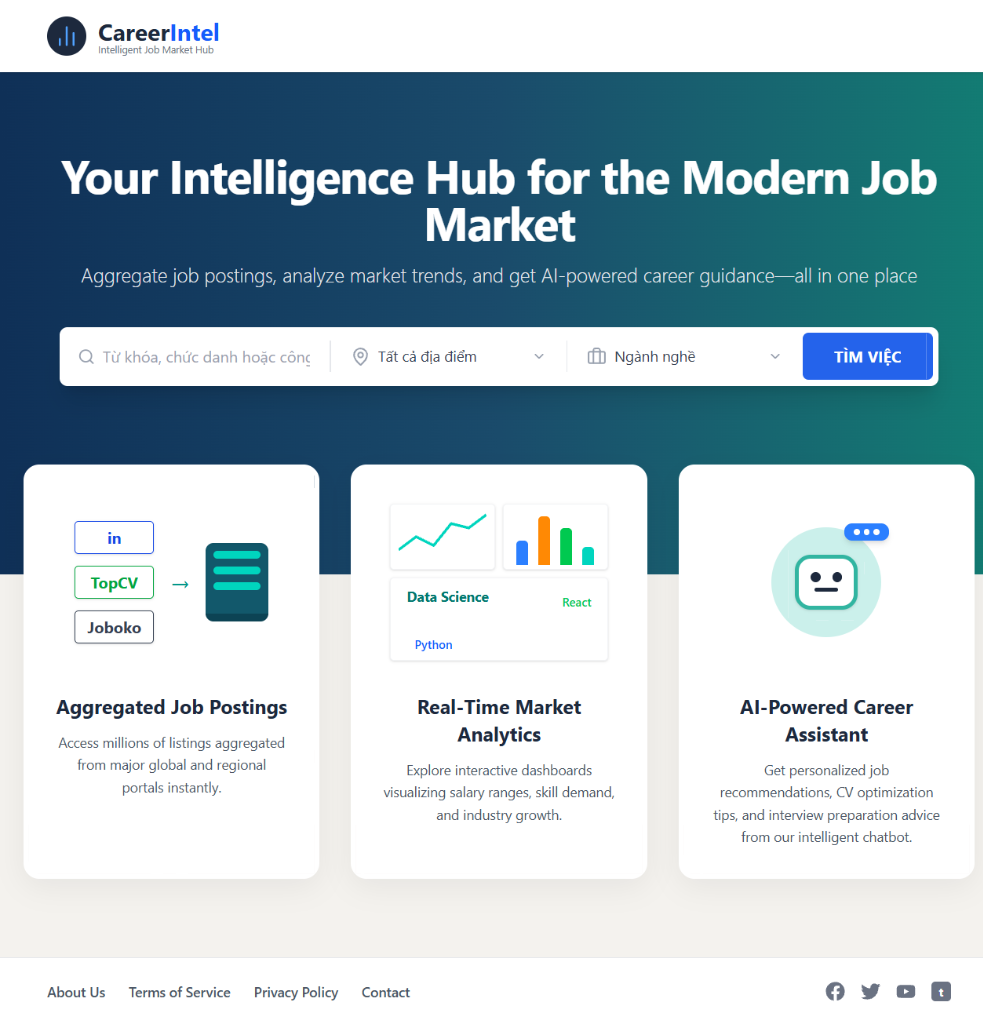
\includegraphics[width=\textwidth]{thesis_1_images/screenshot_homepage.png}
    \caption[Homepage screenshot]{\textbf{Homepage screenshot}: \textmd{Screenshot of the platform's landing homepage UI showing aggregated job searches and platform features.}}
\end{figure}

\noindent The homepage serves as the primary entry point for job seekers. The top navigation provides access to the job search engine, the AI career assistant, market insights, and user profile management. The central search bar enables full-text queries powered by the Elasticsearch cluster (\S3.2), while category cards below expose the 66 standardized job taxonomy tags. The interface is rendered via Next.js Server-Side Rendering for optimized initial load performance.

\newpage

\addcontentsline{toc}{section}{Appendix 2: AI Assistant Interface}
\noindent{\LARGE \textbf{Appendix 2: AI Assistant Interface}\par}
\vspace{0.4cm}
\begin{figure}[H]
    \centering
    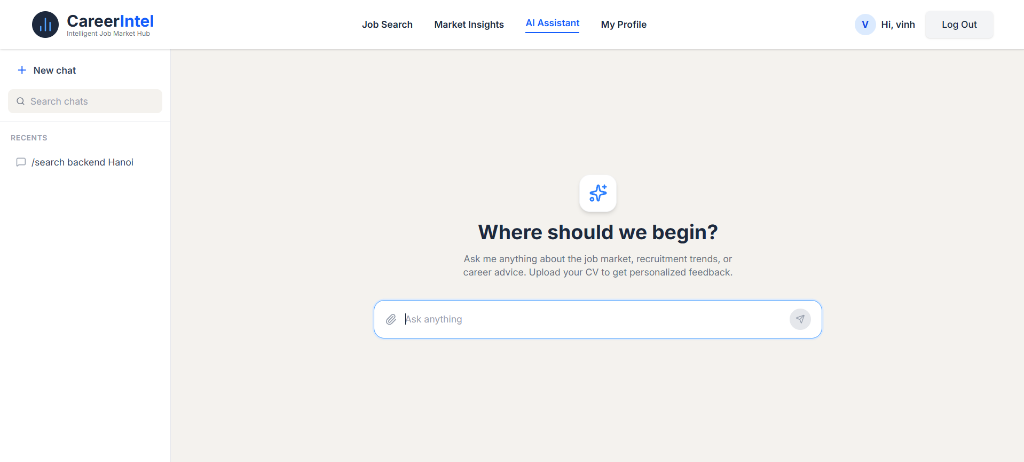
\includegraphics[width=\textwidth]{thesis_1_images/screenshot_ai_assistant.png}
    \caption[AI Assistant interface screenshot]{\textbf{AI Assistant interface screenshot}: \textmd{Screenshot of the interactive SLM-powered career assistant chat interface.}}
\end{figure}

\noindent The AI assistant interface implements the conversational state architecture described in \S3.3.4. The left sidebar displays the conversation history managed through MongoDB embedded documents. The main chat area renders responses from the three QLoRA adapters (\S3.4.2) using the task-type presentation router (\S3.3.5): markdown prose for career coaching, structured tables for interview preparation, and interactive job cards for search results. The file attachment button triggers the asynchronous CV upload pipeline (\S3.3.3).

\newpage

\addcontentsline{toc}{section}{Appendix 3: My Profile Page}
\noindent{\LARGE \textbf{Appendix 3: My Profile Page}\par}
\vspace{0.4cm}
\begin{figure}[H]
    \centering
    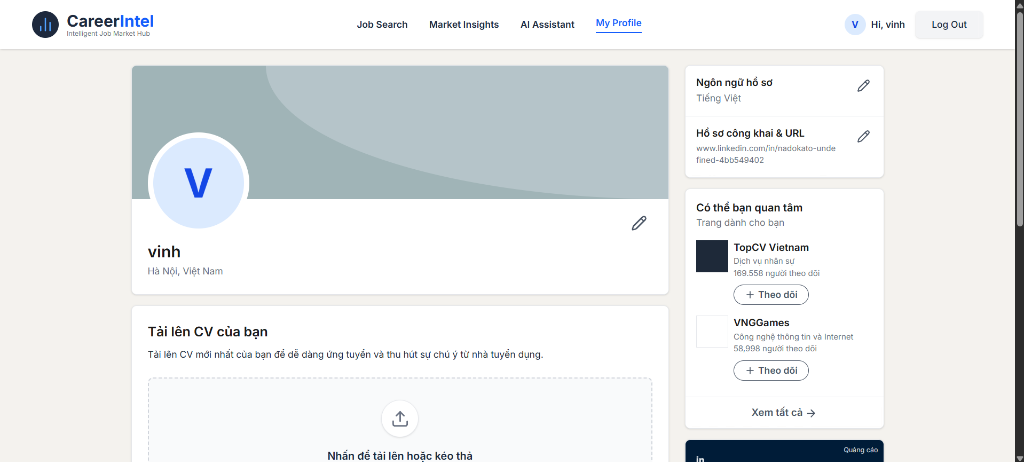
\includegraphics[width=\textwidth]{thesis_1_images/screenshot_my_profile.png}
    \caption[My Profile page screenshot]{\textbf{My Profile page screenshot}: \textmd{Screenshot of the candidate profile management interface showing CV upload and parsed profile details.}}
\end{figure}

\noindent The profile page displays the structured output of the CV extraction pipeline (\S3.1.5.2). After a user uploads a resume, the Celery background worker processes the document through the four-stage transformation (ingestion, text extraction, semantic structuring, and vectorization), and the resulting CanonicalResume JSON is rendered here. The page shows extracted personal information, skills, work experience, and education, alongside the quality score computed by the heuristic scorer (\S3.5.3.2). This data is persisted in Supabase for cross-session retrieval (\S3.2.4).

\newpage

\addcontentsline{toc}{section}{Appendix 4: Market Insights Dashboard}
\noindent{\LARGE \textbf{Appendix 4: Market Insights Dashboard}\par}
\vspace{0.4cm}
\begin{figure}[H]
    \centering
    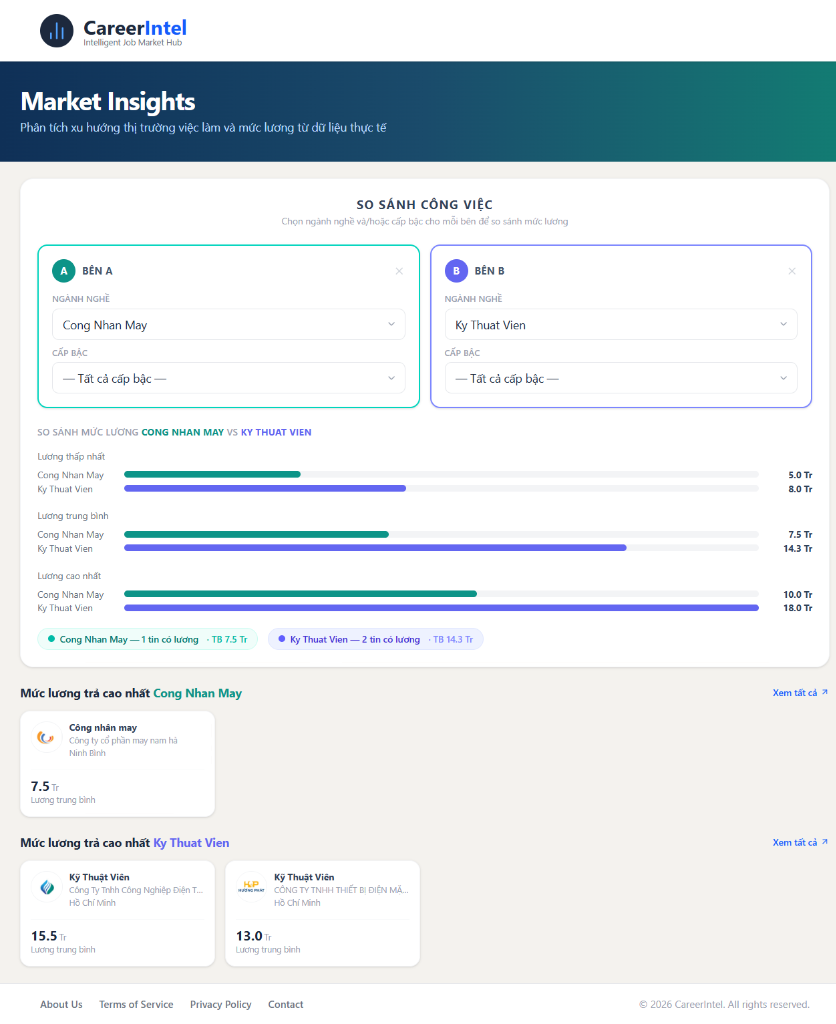
\includegraphics[width=\textwidth]{thesis_1_images/screenshot_market_insights.png}
    \caption[Market Insights dashboard screenshot]{\textbf{Market Insights dashboard screenshot}: \textmd{Screenshot of the job market comparison dashboard illustrating salaries across different roles.}}
\end{figure}

\noindent The market insights dashboard visualizes aggregated analytics derived from the 6,248 normalized job postings indexed in Elasticsearch. The dashboard presents salary distribution comparisons across roles and geographic regions, trending skill demands, and employer hiring activity. These visualizations are computed from the standardized schema fields produced by the heuristic normalization pipeline (\S4.1), enabling job seekers to make data-driven career decisions based on real-time market conditions.

\end{document}